% -*- mode:flyspell; mode:latex -*-
% \documentclass[a4paper,twoside,11pt]{book}
\documentclass[12pt]{article}
\usepackage[latin1]{inputenc}
\usepackage[T1]{fontenc}
\usepackage[english]{babel}
\usepackage{graphicx}
\usepackage{float}
\usepackage{amsmath}
\usepackage{hyperref}
\usepackage{hhline}
\usepackage{subfig}
\usepackage{color}
\usepackage[all]{hypcap}
% \usepackage[normalem]{ulem}  % for striking out
% \usepackage{fancyhdr}
% \pagestyle{fancy}
% \fancyhead[C]{}
% \fancyhead[L] {\it{Mu2e-doc-4555-v1.0} }

\usepackage[square,sort,comma,numbers]{natbib}

% \usepackage[backend=biber, style=numeric-comp, sorting=ynt] {biblatex}

% \addbibresource{mu2e_internal_notes.bib}
% \addbibresource{radiative_muon_capture.bib}
% \addbibresource{radiative_pion_capture.bib}

\newcommand {\red}          {\color{red}}
\newcommand {\blue}         {\color{blue}}

\newcommand {\kmax}         {\mbox{$k_{\rm max}$}}
\newcommand {\mubunch}      {$\mu$Bunch}
\newcommand {\MuMinusEPlus} {\mbox{$\mu^- \rightarrow e^+$}}
\newcommand {\ra}           {\mbox{$\rightarrow$}}

\graphicspath{{figures/}}

\begin{document}

\begin{titlepage}
  \begin{flushright}
    \bf {MU2E/PHYSICS/22262} \\
    version 0.0
    \today
  \end{flushright}

  \vspace{1cm}
  
  \begin{center}
    {\Large \bf Understanding the \kmax\ fits of the RMC spectra} 
    
    \vspace{1cm}
    
    E.Diociaiuti (Roma), M.Mackenzie (Northwestern), P.Murat(FNAL)
    
    % \footnote{\texttt{Fermilab; e-mail: murat@fnal.gov}}
    \vspace{0.3cm}
    
    \vspace{0.8cm}                           
  \end{center}

  \begin{abstract}

    This note summarizes our effort to understand published results
    on the endpoint determination of the Radiative Muon Capture (RMC)
    spectra. 
%
    We conclude that internal inconsistencies found in the literature make
    it difficult to rely on the results of other experiments when predicting
    RMC background to the search of \MuMinusEPlus\ conversion process.

    However, we establish that uncertainties on the RMC endpoint
    published by the TRIUMF RMC spectrometer group are overestimated
    by a factor of about 4-5, with the real uncertainty of the measurements
    being in the range of 0.4-0.5 MeV, rather than 1.5-2 MeV.

    Using $\chi^2$ fit results in biased estimates of the RMC photon
    spectrum endpoints, so the likelihood fit should be used.
    
    To reliably predict RMC background to  \MuMinusEPlus, Mu2e needs to have
    its own measurement of the endpoint of the RMC photon spectrum on Al.
    
  \end{abstract}

\end{titlepage}
% \frontmatter
% \chapter*{Abstract}
%
% \addcontentsline{toc}{chapter}{Abstract}
%
% \mainmatter
%
{\tableofcontents}

%%%%%%%%%%%%%%%%%%%%%%%%%%%%%%%%%%%%%%%%%%%%%%%%%%%%%%%%%%%%%%%%%%%%%%%%%%%%%%%
%\chapter{Calibration}
%%%%%%%%%%%%%%%%%%%%%%%%%%%%%%%%%%%%%%%%%%%%%%%%%%%%%%%%%%%%%%%%%%%%%%%%%%%%%%%
\section{ RMC as a background to \MuMinusEPlus\ conversion search }
% 
% \begin{figure}[H]
%   \includegraphics[width=1.05\textwidth]{figures/png/beam_flash_electron_momentum} 
% 
%   \caption{
%    momentum spectrum of the beam flash electrons
%   }
% \end{figure}

Radiative muon capture (RMC) is one of the most important backgrounds to the search for
\MuMinusEPlus\ conversion on nuclei. In case of the Mu2e target of choice, aluminum,
RMC is also the most uncertain one: the expected signal $e^+$ energy, E = 92.32 MeV,
is close enough to the endpoint of the RMC spectrum on aluminum,
$90 \pm 2$ MeV \cite{RMC_1999_PhysRevC.59.2853}, so variations of the endpoint
energy within the experimental errors could result in significant changes
in the RMC background expectations.
%
%% We note that the uncertainty in the RMC background expectations is mostly due to the
%% published experimental uncertainty of 2 MeV - 
The Mu2e energy resolution of about 300-400 keV
is small compared to a $\sim$ 3 MeV difference between the expected signal energy
and the maximal energy of a positron coming from a conversion of a RMC photon.
However, given the published 2 MeV uncertainty on the RMC spectrum endpoint the two 
numbers are just about 1.5 standard deviation apart, so understanding of the
experimental uncertainty on \kmax\ becomes quite important.

Fortunately, measurements of the photon spectra on nuclei published 
by the TRIUMF RMC spectrometer group in \cite{RMC_1992_PhysRevC.46.1094},
\cite{RMC_1999_PhysRevC.59.2853} provide sufficient information for readers
to reproduce the published photon spectrum endpoints, and in this note
we report on our attempt to do so.

The endpoint of the RMC photon spectrum is determined using the closure
approximation model \cite{RMC_1979_CERN_REF-TH-2967}.
In this model, the photon spectrum is fully defined by a single parameter,
the photon spectrum endpoint energy \kmax:
$$
   {dN \over dx} = {e^2 \over \pi} {\kmax^2 \over {m_\mu^2}}  (1-x) (1-2x+2x^2) x (1-x)^2
$$
where $x = k/\kmax$.

We use published parameterizations of the TRIUMF RMC spectrometer response
to convolute them with the closure approximation spectra, fit the experimental data,
determine the best \kmax\ values and the corresponding fit uncertainties
for different nuclei, and compare the fit results to the published values.

%%%%%%%%%%%%%%%%%%%%%%%%%%%%%%%%%%%%%%%%%%%%%%%%%%%%%%%%%%%%%%%%%%%%%%%%%%%%%%%
\section { Parameterization of the Detector Response}


Published are the measured data. To compare them to the model predictions,
one needs to know how the theoretical spectrum is modified by the detector
response, i.e. know the detector response.

The detector response D(E,E') describes the probability of detect a photon
 of true energy E with a reconstructed energy E'.

In the following the two detector responses published respectively in 
 \cite{RMC_1992_PhysRevC.46.1094} and \cite{RMC_1998_PhysRevC.58.1767}
 are in detail described.
 Both are determined using the GEANT Monte Carlo simulation using monoenergetic photons
 in a energy range of 50-140 MeV and fitted to a analytic parametrization.

\subsection { 1992 Detector response parametrization}
The parametrization represent a Gaussian distribution with exponential low- and
 high-energy tails. In order to reproduce the low-energy tails for high-energy photons a second Gaussian is added to the fuction for photon energy E>60 MeV.
The fuction form is:
\begin{equation}
\text{D(E,E')}= \left\{
\begin{array}{ll}
                \text{A exp}\left[-\frac{1}{2\sigma_0^2}(E'-E_o)\right]+
                \text{F exp}\left[-\frac{1}{2\sigma_3^2}(E'-E_3)^2\right]
 \quad E_1<E'<E_2 \\
                \text{B exp}\left[-\frac{1}{\sigma_1}(E_1-E') \right]+
                \text{F exp}\left[-\frac{1}{2\sigma_3^2}(E'-E_3)^2\right]
 \quad E'<E_1      \\  
                \text{C exp}\left[-\frac{1}{\sigma_2}(E'-E_2)\right]+
                \text{F exp}\left[-\frac{1}{2\sigma_3^2}(E'-E_3)^2\right]
 \quad E'>E2     
 \end{array}
 \right\}
\end{equation}
 
where $E_1=E_0 - \frac{\sigma_0^2}{\sigma_1}$, $E_2 =E_0 + \frac{\sigma_0^2}{\sigma_2}$,
 $B=\text{A exp}\left[-\frac{\sigma_0^2}{2\sigma_1^2}\right]$, 
 $C=\text{A exp}\left[\frac{\sigma_0^2}{2\sigma_2^2}\right]$. 

The other parameters have a polynomial dependence to the photon energy like:
\begin{equation}
f(E)= P_0+P_1E+P_2E^2+P_3E^3
\end{equation} 
the coefficients are reported in table~\ref{tab:coefficients1} and ~\ref{tab:coefficients2} .
\begin{table}[!h]
\begin{center}
\begin{tabular}{| c | c | c | c | c | }
\hline
Parameter & $P_0$ (MeV)& $P_1$ & $P_2$ (MeV)$^{-1}$ \\ \hline
$\sigma_0$ & -0.5836 & 0.0352 & \\ \hline
$\sigma_1$ & -5.879 & 0.1653 & -5.149$\times 10^{-4}$ \\ \hline
$\sigma_2$ & 1.596 & -0.03859 & 3.883$\times 10^{-4}$ \\ \hline
$\sigma_3$ & -47.80 & 1.010 & -4.406$\times 10^{-3}$ \\ \hline
E$_3$ & 1.068 & 0.7507 & \\ \hline
E$_0$ (E>60) & -1.161 & 0.9481 & 1.724$\times 10^{-3}$ \\ \hline
E$_0$ (E<60) & 22.73 & 0.1995 & 5.993$\times 10^{-3}$ \\ \hline

\end{tabular}
\end{center}
\caption{Coeffiecients of the polynomial energy dependece of the response fuction parameters\label{tab:coefficients1}}
\end{table}

\begin{table}[!h]
\begin{center}
\begin{tabular}{| c | c | c | c | c | c |}
\hline
Parameter & $P_0$ & $P_1$ (MeV)$^{-1}$ & $P_2$ (MeV)$^{-2}$  & $P_3$ (MeV)$^{-3}$\\ \hline
A & 3.259$\times 10^{-4}$ & -4.120$\times 10^{-4}$ & 1.015$\times 10^{-5}$ & -4.05$\times 10^{-8}$  \\ \hline
F/A & -0.1337 & 2.828$\times 10^{-3}$ & -9.701$\times 10^{-6}$ & \\ \hline
\end{tabular}
\end{center}
\caption{Coeffiecients of the polynomial energy dependece of the photon acceptance parameters\label{tab:coefficients2}}
\end{table}

In Fig.~\ref{fig:parameterDependance} the photon energy dependence of the parameters of the detector response fuction are plotted.
\begin{figure}[!h]
 \begin{center}
 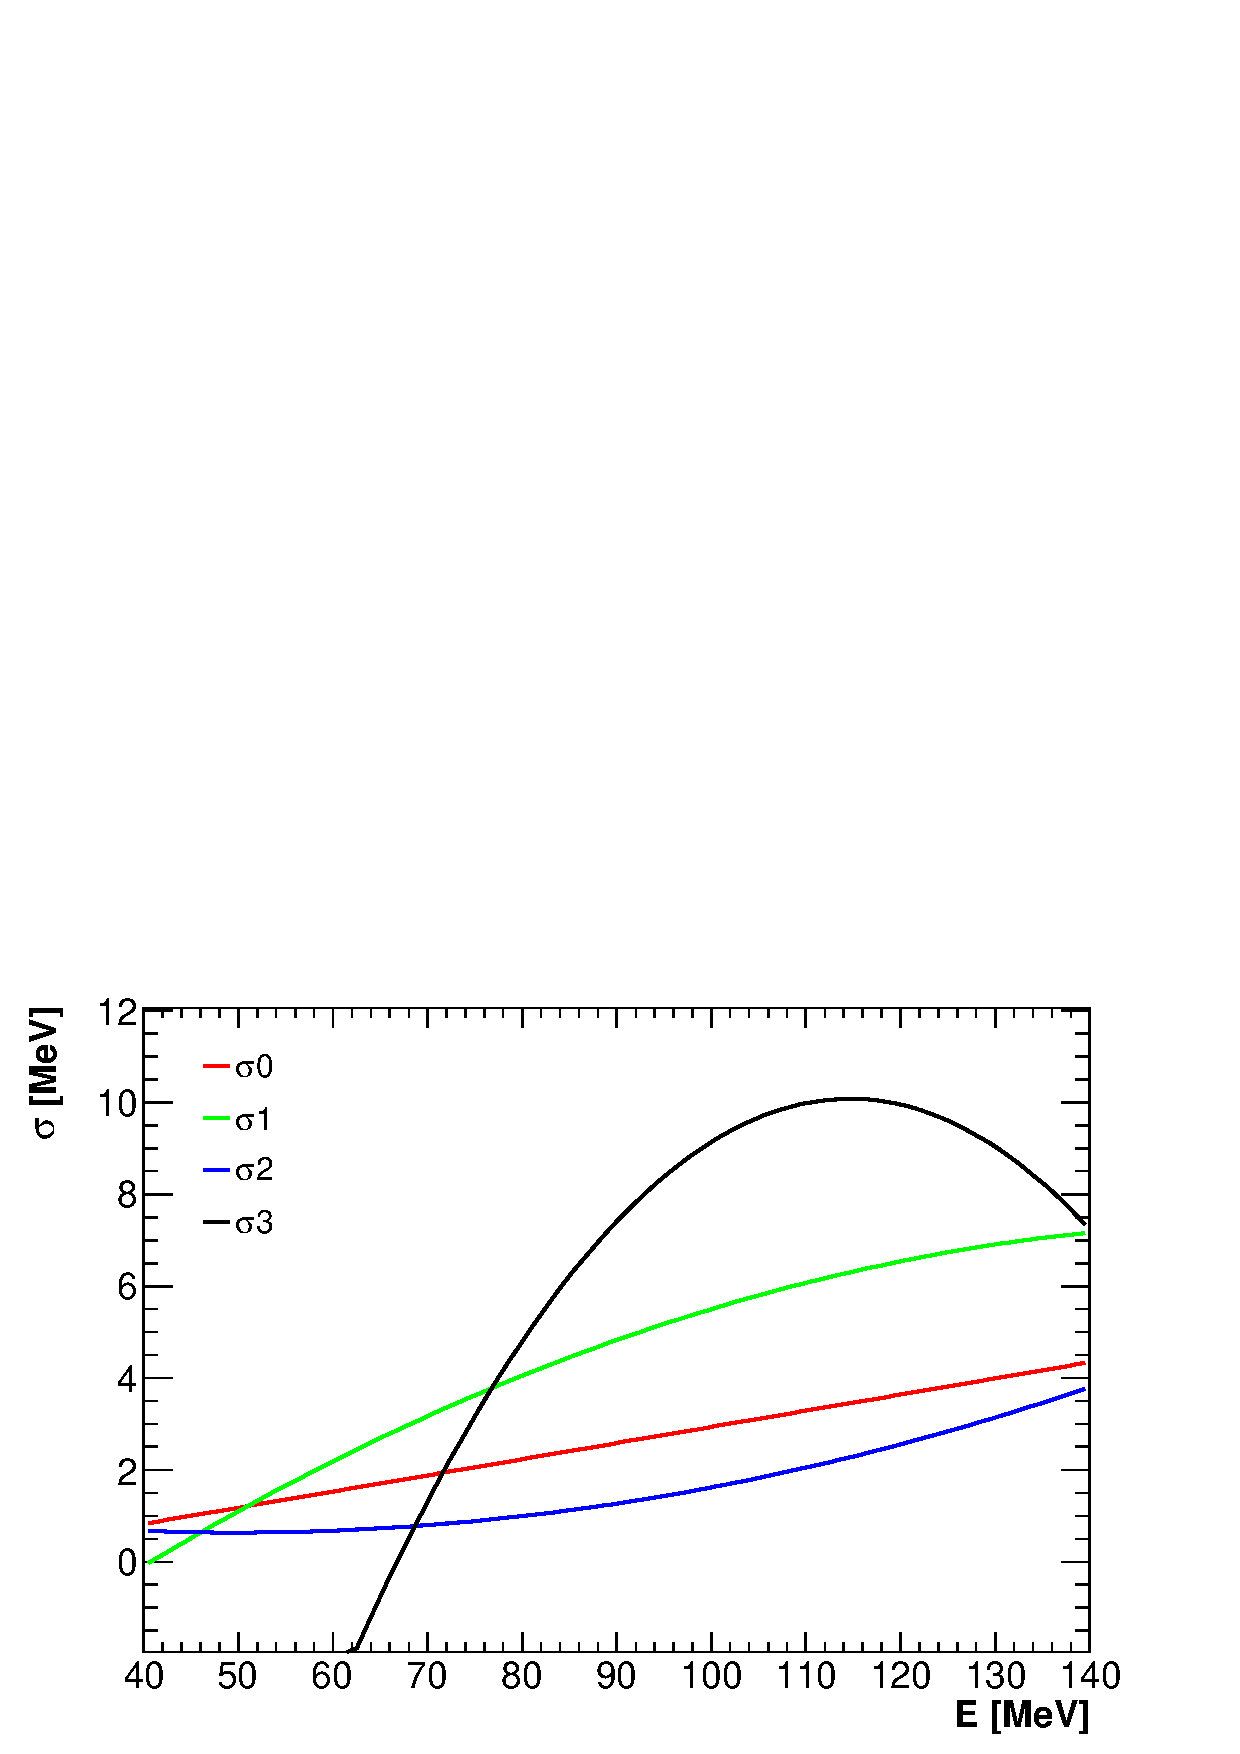
\includegraphics[width=0.33\columnwidth]{png/sigmas92.png} 
 \includegraphics[width=0.33\columnwidth]{png/A_FoverA92.png} 
 \includegraphics[width=0.33\columnwidth]{png/E092.png} 
 \end{center}
 \caption{Energy dependence of the different parameter defining the detector response}
 \label{fig:parameterDependance}
 \end{figure}


Some examples of the detector response at different energies, namely 50 MeV , 70 MeV , 90 MeV, and 110 MeV,
 are reported in Fig.~\ref{fig:92ResponseExample}.\\
As previously described, for photon energies E>60 MeV, the low-energy tails are well evident.

\begin{figure}[!h]
\centering
\includegraphics[width =\textwidth]{png/Resp_example92.png}
\caption{1992 detector response parametrization for different photon energies}
\label{fig:92ResponseExample}
\end{figure}


\subsection { 1998 Detector Response }

Because of differences in the triggers used in this later work the detector response results slightly different.
The fuction used to describe the detector response through  a Gaussian peak with logaritmic low-energy  and an exponetial high-energy tail:

\begin{equation}
  D(E,E')= \left\{
    \begin{array}{ll}
      \gamma ln(x)/x          \qquad E' \leq (E_0-\sigma_0) \\
      Ae^{-(E'-E_0)^2/2\sigma_0^2} \qquad E0-\sigma_0<E'<(E_0-\sigma_0^2/\sigma^2) \\
      Ae^{-(E'-E_0)/2\sigma_2}    \qquad E' \geq (E_0+\sigma_0^2/\sigma_2)
    \end{array}
  \right\}
\end{equation}

The quantity $\beta$  allows the matching of the low-side and core of the distribution at E'=$E_0-\sigma_0$.

The quantity $x$ is defined as 
$$x= \frac{\alpha- E}{\alpha -37 \text{ MeV}}$$.
Also in this case the parameters $\alpha,A,E_0,\sigma_0,\sigma_2$ have a polynomial dependence on the photon energy that can be parametrized as:

\begin{equation}
\alpha= a+0+a_1y+a_2y^2+a_3y^3
\end{equation}

where $y= (E-60 \text{MeV}/60 \text{ MeV})$/


The  coefficient of the parameters are reported in Tab.~\ref{tab:param98}
\begin{table}[!h]
\begin{center}
\begin{tabular}{| c | c | c | c | c | c | }
\hline
Parameter & $a_0$ & $a_1$ & $a_2$ & $a_3$ \\ \hline
$\alpha$ & 56.1 &62.5 & -0.826 & 0.0  \\ \hline
A & 9.41$\times 10^{-4}$ & 2.61$\times 10^{-3}$ &0.27 $\times 10^{-2}$ &0.835$\times 10^{-3}$   \\ \hline
$E_0$ & 54.4 & 57.7 & -0.315 &0.0 \\ \hline
$\sigma_0$ & 2.03 &10.4 &1.25 & -0.428\\ \hline
$\sigma_2$ & 0.786 & 0.508 & 0.425 & -0.164\\ \hline

\end{tabular}
\end{center}
\caption{Coeffiecients of the polynomial energy dependece of the response fuction parameters\label{tab:param98}}
\end{table}

In Figure~\ref{fig:parameters98} the different parameters of the response fuction are plotted as a function of the photon energy.


\begin{figure}[!h]
 \begin{center}
 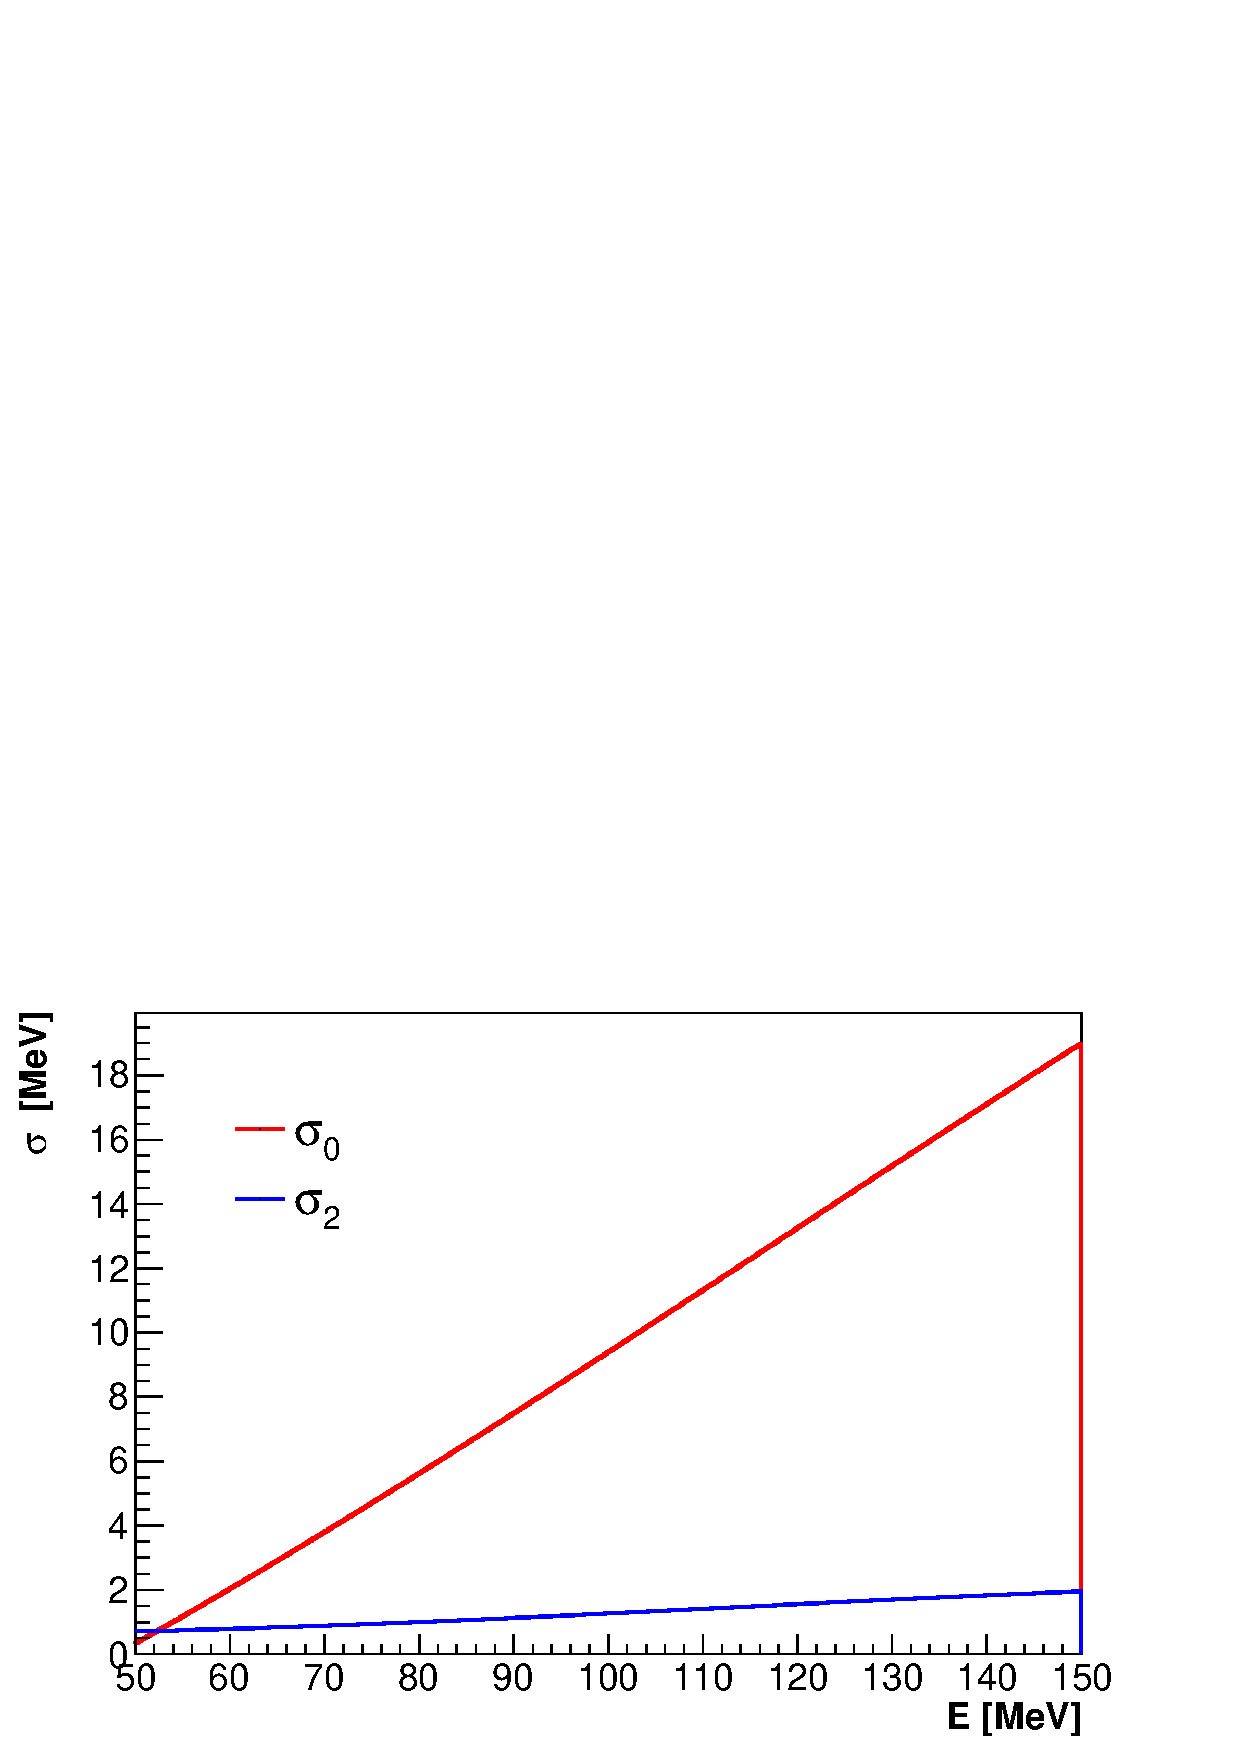
\includegraphics[width=0.49\columnwidth]{png/sigmas98.png} 
 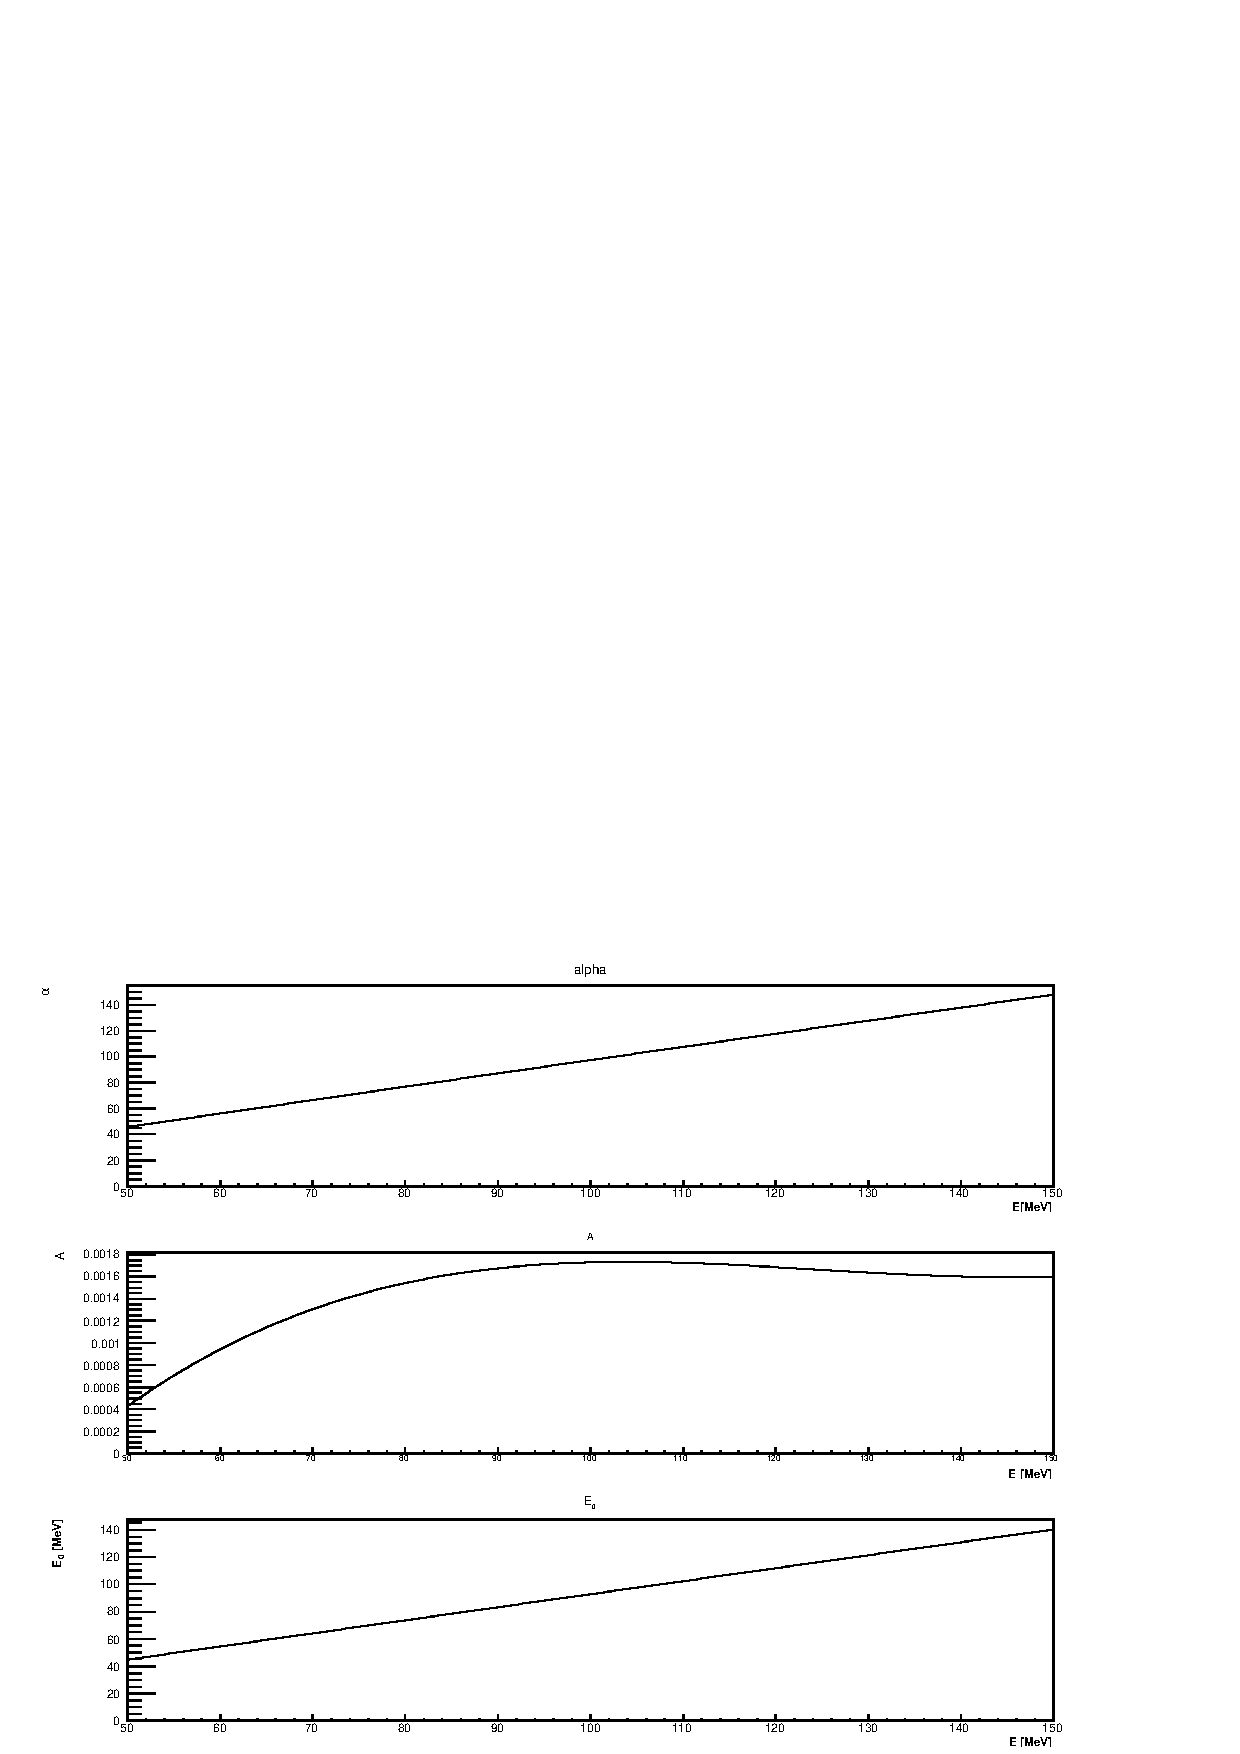
\includegraphics[width=0.49\columnwidth]{png/par98.png} 
 \end{center}
 \caption{Energy dependence of the different parameter defining the detector response}
 \label{fig:parameters98}
 \end{figure}

In  Figure~\ref{fig:response98} the detector response is plotted for different photon energies, even if the distributions result two times wider with respect to the one of 1992 no explanation is given to justify this change.  %a difference in the shape of the distribution is clearly evident

\begin{figure}[!h]
\centering
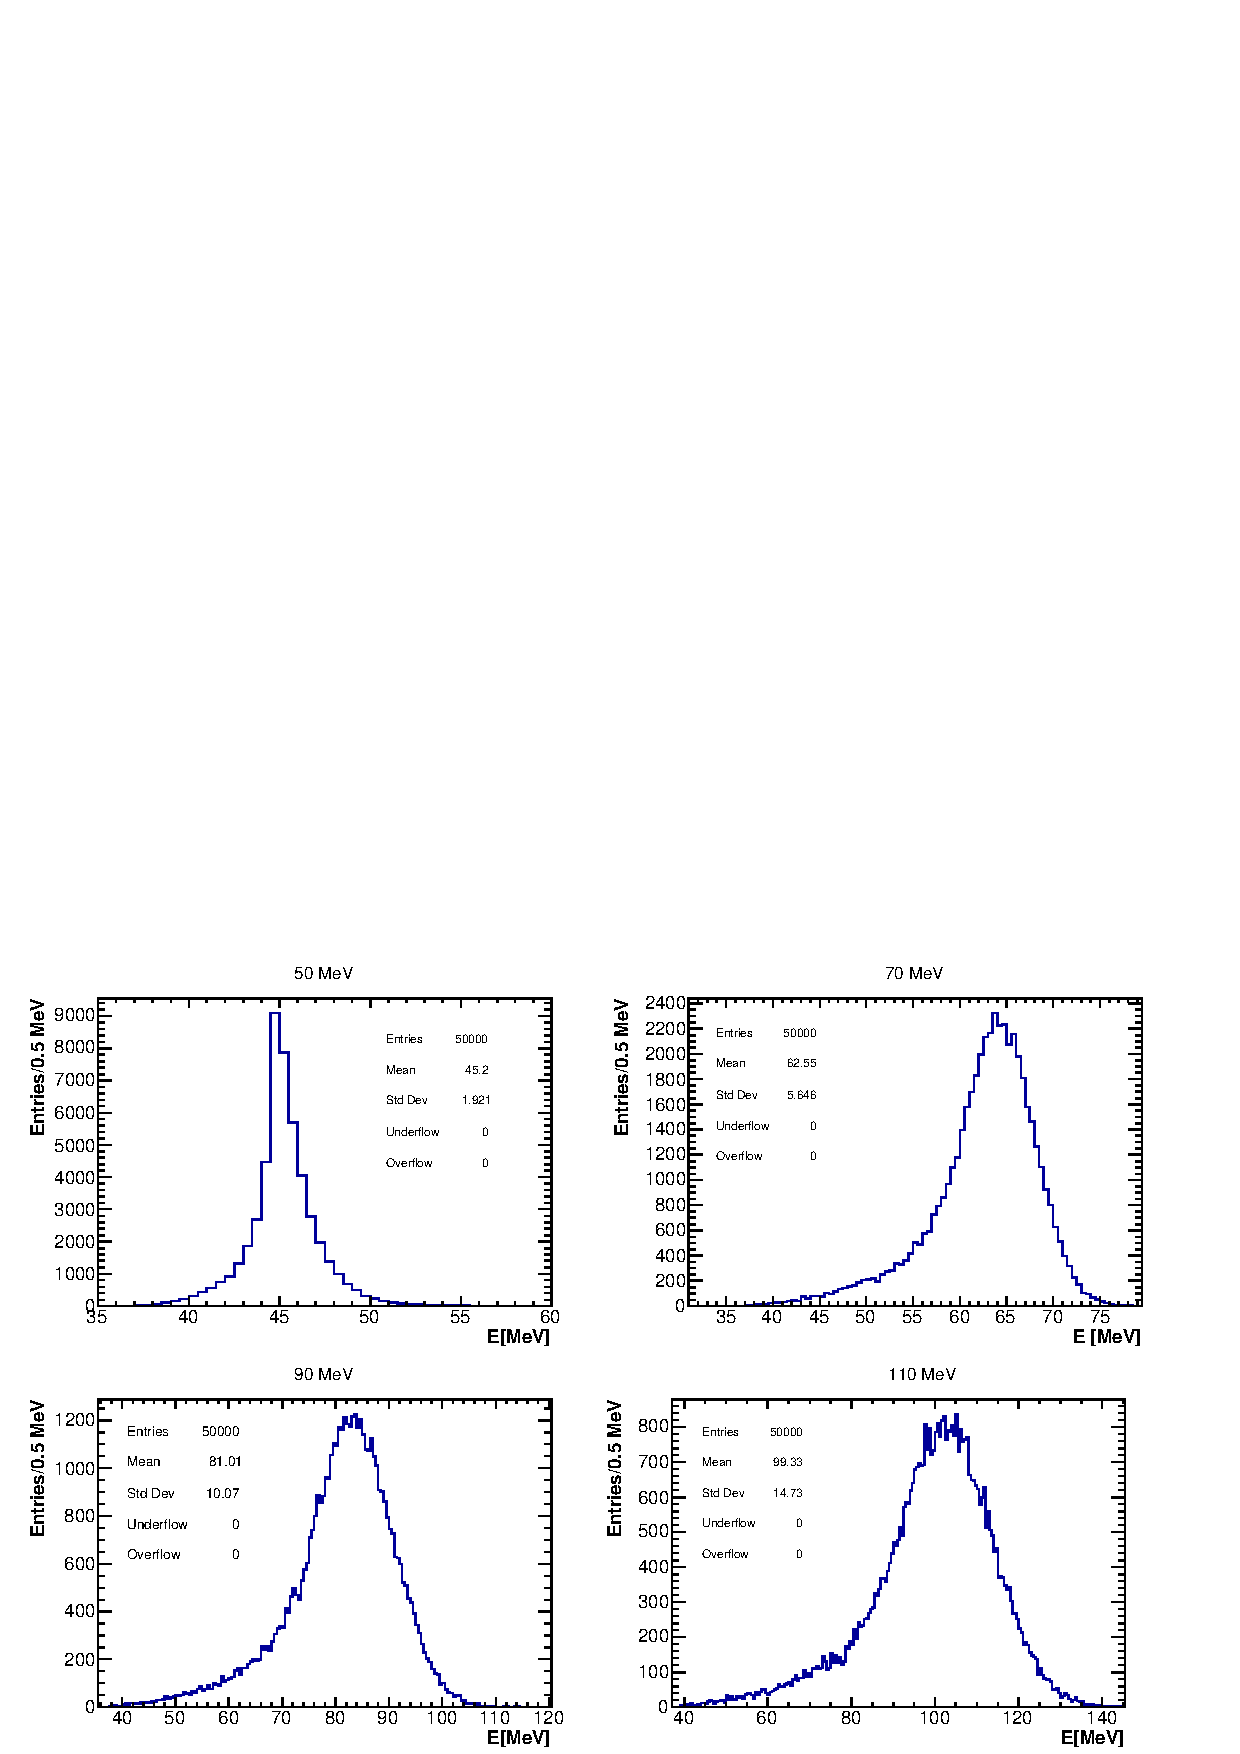
\includegraphics[width =\textwidth]{png/Resp_example98.png}
\caption{1998 detector response parametrization for different photon energies}
\label{fig:response98}
\end{figure}

In Figure~\ref{fig:shapecomp} the shape comparison of the two detector responses at 90 MeV (left) and the peaks of the detector responses as a function of the photon energies (right) are reported. The linearity of the two detector responses is similar.

\begin{figure} [!h]
\centering
\includegraphics[width=0.49\columnwidth]{png/detRespinsieme.png}
\includegraphics[width=0.49\columnwidth]{png/9298fit.png}
\caption{Left: comparison of the shape of the detector response to a 90 MeV photon. Right:peak of the detector response as a fuction of the photon energies }
\label{fig:shapecomp} 
\end{figure}

We check how well different parameterizations of the detector response describe the 
calibration peak at 129.4 MeV obtained from $\pi^{-}p \rightarrow \gamma n$ on LH$_{2}$ reported in the 1992 
A good agreement is shown in Figure~\ref{p004}(left) between data and  1992 response function, while the 1998 article has a completely different behaviour.\\

\begin{figure}[!h]
 \begin{center}
 \includegraphics[width=0.49\columnwidth]{png/RPC_Data_vs_1992_Response.png} 
 \includegraphics[width=0.49\columnwidth]{png/RPC_Data_vs_1998_Response.png} 
 \end{center}
 \caption{Response function of the 1992 article (left) and 1998 article (right) compared with the 129.4 MeV line from RPC on LH$_{2}$}
 \label{p004}
 \end{figure}

 In the 1998 article  however to validate  the detector response, the Radiative Pion Capture on $^{12}$Ca  is compared with the simulated data and a good agreement is reported as shown in Figure~\ref{fig:art9}.

\begin{figure}[!h]
 \begin{center}
 \includegraphics[width=0.45\textwidth]{png/RPC12Ca.png} 
 \end{center}
 \caption{RPC spectrum from  $\pi^{-}p \rightarrow \gamma n$ on  $^{12}$Ca compared to the simulated data }
 \label{fig:art9}
 \end{figure}

%%%%%%%%%%%%%%%%%%%%%%%%%%%%%%%%%%%%%%%%%%%%%%%%%%%%%%%%%%%%%%%%%%%%%%%%%%%%%%%
\section { Input data for the \kmax\ fits}

The digitized figures from references \cite{RMC_1992_PhysRevC.46.1094,RMC_1999_PhysRevC.59.2853}
are used as input data for our fits. We assume that the published spectra plot numbers of events
per bin and that the errors used in the fits are purely statistical.

To check the first assumption, we show in Figure \ref{fig:digitization_accuracy_x_y_left} the accuracy
of digitizing the energy bin centers for a digitized plot. It is calculated as the difference between 
the digitized bin center and the expected bin center, N+0.5.
Figure \ref{fig:digitization_accuracy_x_y_right} shows the accuracy of digitizing the bin contents.
Plotted is the difference between the digitization and the closest integer, where the assumption is that 
each bin contains an integer number of entries. The digitization accuracy of the bin contents has
a standard deviation close to 0.1 and a mean also close to 0.1, which could be due to a
mis-calibration of the Y axis in the digitization of the plot.

\begin{figure}[htbp]
  \begin{center}
    \subfloat[\label{fig:digitization_accuracy_x_y_left}]{ %
    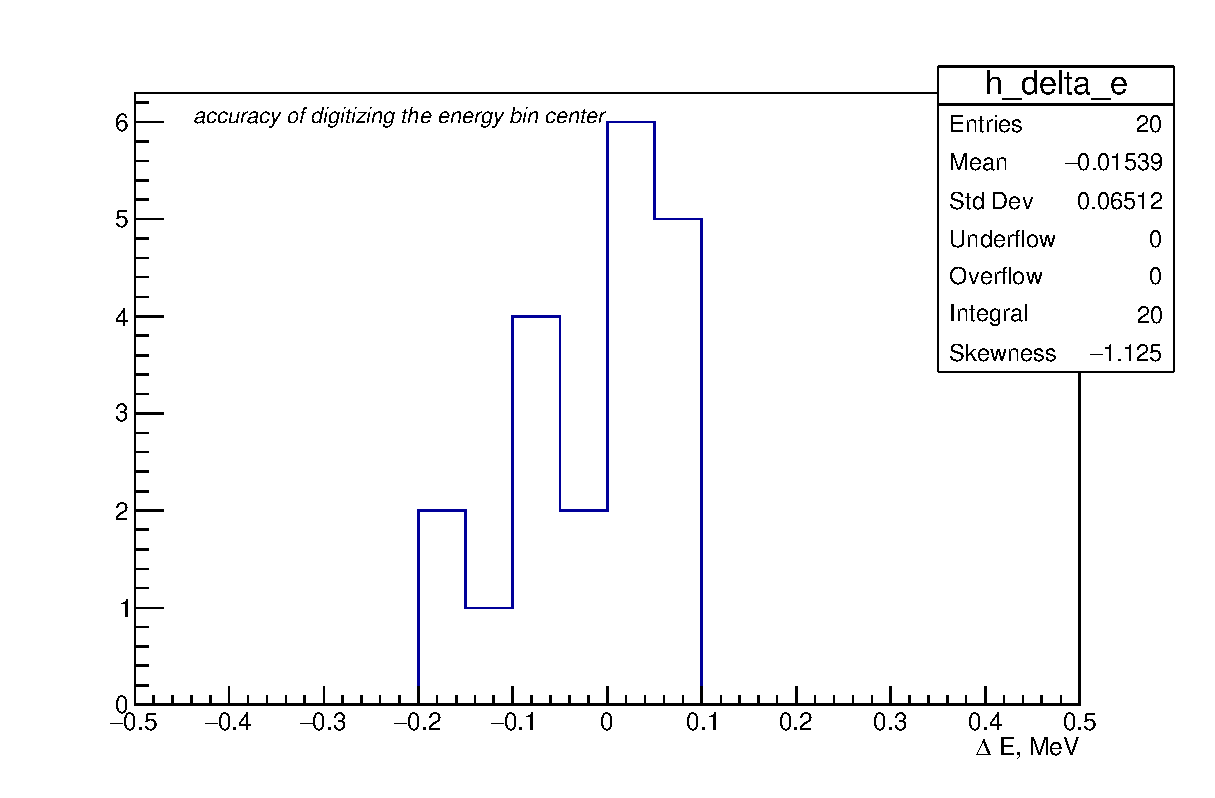
\includegraphics[width=0.49\columnwidth]{png/digitization_accuracy_de}}
    \subfloat[\label{fig:digitization_accuracy_x_y_right}]{ %
    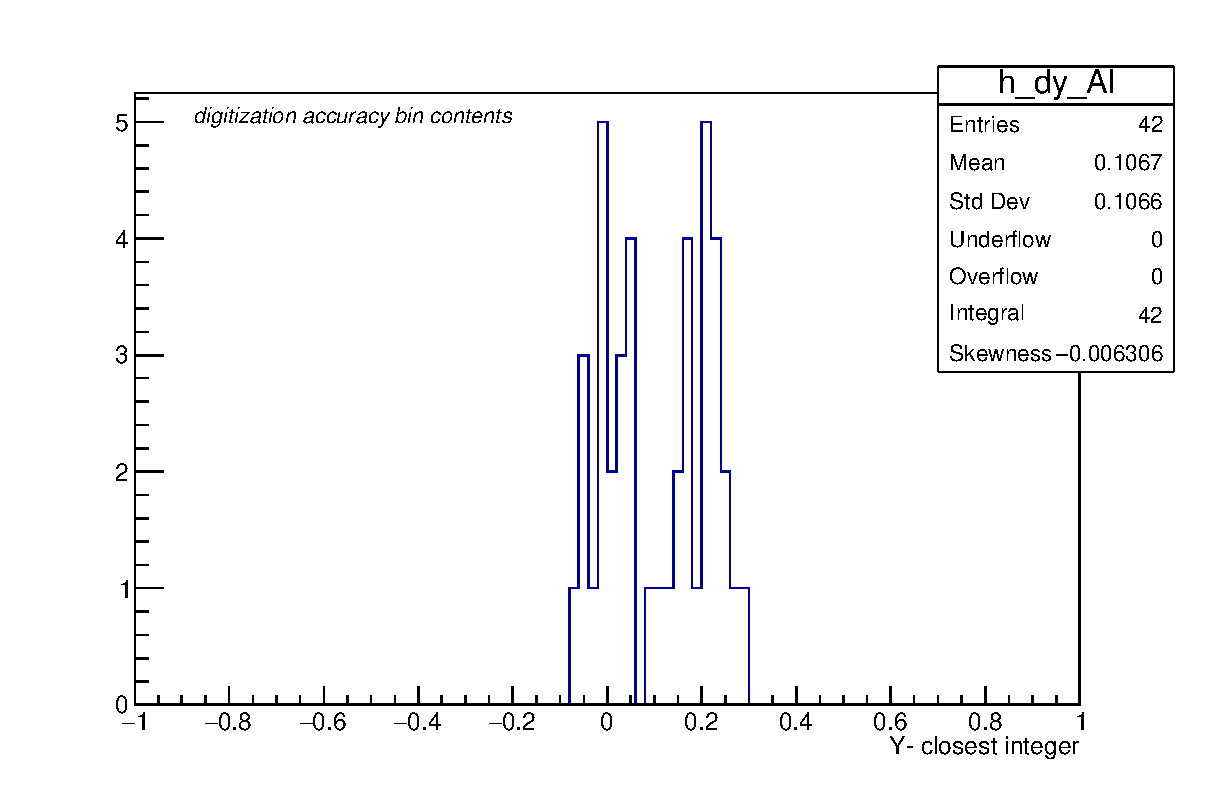
\includegraphics[width=0.49\columnwidth]{png/digitization_accuracy_Al_1992_dy} }
  \end{center}
  \caption{
    (a): accuracy of digitizing the histogram bin centers
    (b): digitization accuracy of the bin content
  }
  \label{fig:digitization_accuracy_x_y}
\end{figure}

The distribution in figure \ref{fig:digitization_accuracy_error_bars} plots the residuals
$\Delta_Y = 0.5((Y+\sigma_Y) + (Y-\sigma_Y)) - \sqrt{Y}$ for one of the digitized plots.
It confirms the assumption that the error bars on the plots are purely statistical.

\begin{figure}[htbp]
  \begin{center}
    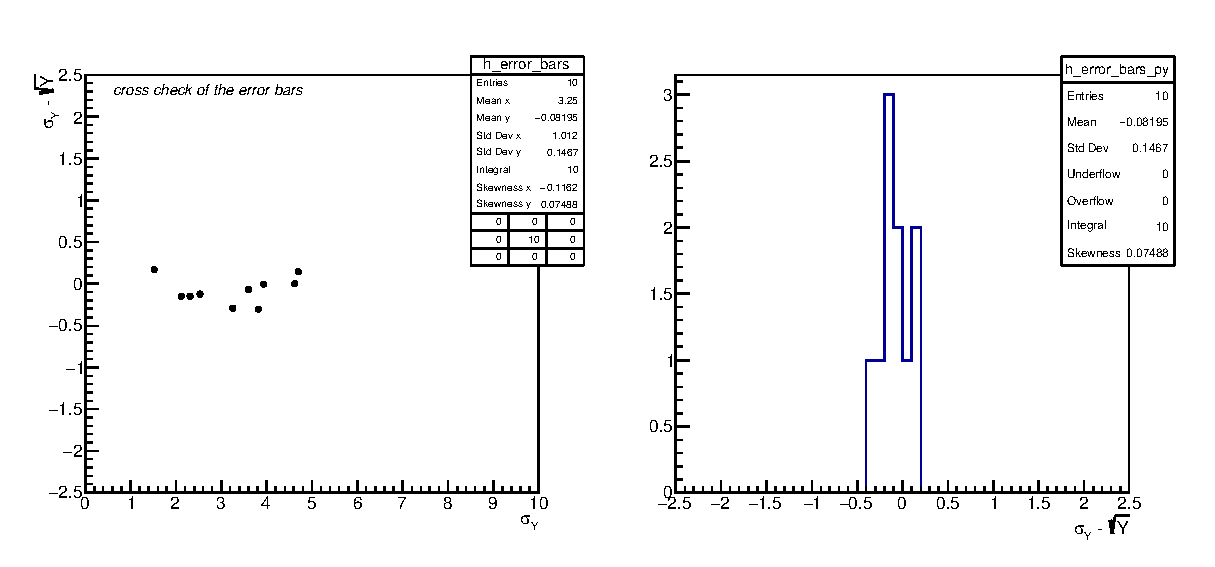
\includegraphics[width=0.99\columnwidth]{png/digitization_error_bars} 
  \end{center}
  \caption{
    left: error bar residuals, $\Delta_Y$, vs the digitized error bars
    right: y-projection of the left histogram
  }
  \label{fig:digitization_accuracy_error_bars}
\end{figure}


\section { Systematic uncertainty on the energy scale}

The energy scale of the TRIUMF RMC spectrometer has been calibrated using the
radiative pion capture (RPC) on hydrogen \cite{RMC_1992_WRIGHT_1992_249}.
Figure \ref{fig:1992_photon_spectrum_calibration} shows the measured RPC spectrum
overlayed with the simulation results. The histogram bin width
is 500 keV, and one can see that the systematic uncertainty in the reconstructed
photon energy does not exceed one bin, i.e. 0.5 MeV. Differences near 80 MeV
more likely reflect a systematics in the acceptance calculation.

\begin{figure}[htbp]
  \begin{center}
    \includegraphics[width=0.7\columnwidth]{png/1992_TRIUMF_RMC_facility_fig_9_photon_spectrum_calibration} 
  \end{center}
  \caption{
    RPC spectrum on hydrogen measured at the TRIUMF RMC spectrometer \cite{RMC_1992_WRIGHT_1992_249}.
    In the region of the RPC peak, the systematic uncertainty in the reconstructed photon energy does
    not exceed one bin, i.e. 500 keV.
  }
  \label{fig:1992_photon_spectrum_calibration}
\end{figure}

%%% Local Variables:
%%% mode: latex
%%% TeX-master: "."
%%% End:

%%%%%%%%%%%%%%%%%%%%%%%%%%%%%%%%%%%%%%%%%%%%%%%%%%%%%%%%%%%%%%%%%%%%%%%%%%%%%%% 
%%% Local Variables:
%%% mode: latex; mode: flyspell
%%% TeX-master: "."
%%% End:

\section { Fits }

To fit the endpoint energy for a given data spectrum, closure approximation spectra were convolved with a detector
response function using $\kmax$ values between 80 MeV and 100 MeV.
%% convolved spectra were generated for $\kmax$ values between 80 MeV and 100 MeV using both detector response functions.
Each convolved spectrum was scaled to minimize the $\chi^2$ and then the negative log likelihood ($\mathcal{L}$).
%%, where the latter is able to take into account empty bins in the data while the former cannot. 
For the $\mathcal{L}$ minimization, the convolved spectrum value in each bin was taken as the mean 
of a Poisson distribution in this bin.
%% The scale factors to minimize the $\chi^2$ and $\mathcal{L}$ fits were derived by:

%% $$f_{Poisson}(N;x_i) = \frac{x_i^N e^{-x_i}}{N!}$$
%% $$\chi^2 = \sum^N_{i=1} (\frac{A*x_i - y_i}{\sigma_i})^2; \mathcal{L} = -\sum^N_{i=1}log(f_{Poisson}(y_i;A*x_i))$$
%% $$\frac{\partial \mathcal{L}}{\partial A} = 0 \rightarrow A_{\mathcal{L}} = \frac{\sum^N_{i=1} y_i}{\sum^N_{i=1} x_i} $$
%% $$\frac{\partial \chi^2}{\partial A} = 0 \rightarrow A_{\chi^2} = \frac{\sum^N_{i=1} \frac{x_i*y_i}{\sigma_i^2}}{\sum^N_{i=1} \frac{x_i^2}{\sigma_i^2}} $$

%% \noindent
%% where $x_i$ is the predicted value corresponding to data $y_i$ for a given endpoint value.

The distribution of $\chi^2$ and $\mathcal{L}$ values as a function of the endpoint energy were each fit to a parabola near 
their minima to find the best fit endpoint energy. The estimated uncertainty on the endpoint energy is then
defined by $\Delta \chi^2 = 1$ and $\Delta \mathcal{L} = \frac{1}{2}$. This was done using both published detector response
functions, an example fit using the 1992 detector response function
and the 1992 aluminum data is shown in Figure \ref{fig:1992AlFits}. 

The fit $\kmax$ values for all 
datasets and both detector response functions are shown in Figures \ref{fig:ChiSq} and \ref{fig:NLL}, and the $\chi^2$/DOF
distributions are shown in Figure \ref{fig:ChiSqOfFits}. 
%% Should we include the Chi^2 for the NLL fit? Should we define what this means?
%% See Fitter::DoBinnedLikelihoodFit(bool extended) where defines the chi^2 using the data
%% and likelihood function. So straightforward chi^2 with errors from spectrum?
The $\chi^2$/DOF peaks around 1 for the 1998 detector response 
function and does not have the expected shape for the 1992 detector response function. Figure \ref{fig:compareFits}
shows the difference between the $\mathcal{L}$ and the $\chi^2$ fits for both detector response functions.
Figure \ref{fig:ToyFitErrs} shows the errors in fitting toy data generated with
an endpoint energy of 90 MeV. The toy fits shows that the expected difference between the $\chi^2$ and $\mathcal{L}$ fits 
is around 0.5 MeV. The difference between the two fits for the data is around 1 MeV for the fits using the 1998 detector 
response function and around 3 MeV when using the 1992 detector response function, consistent with the 1992 detector response 
not describing the data well. 

A possible source of the discrepancy between the $\chi^2$ and $\mathcal{L}$ fits is a small background 
in the high energy region of the data, which would skew the $\mathcal{L}$ fit $\kmax$ values up due to the high weight they would hold for deviating
from the convolved spectra. In the data spectrum shown in Figure \ref{fig:1992AlFits} there appears to be 3 high energy events above 95 MeV
not consistent with the expected spectrum. One could account for a background like this by removing the top 0.5\% of the data and refitting the remaining
data. Figure \ref{fig:compareFitsTopCut} shows the difference between the fits after this cut on the data, where the 
mean difference is now around 2 MeV for the 1992 detector response function, which is still inconsistent with expectations from
the toy MC studies, and around 0.5 MeV for the 1998 detector response function, which is consistent with the toy MC studies.
The toy MC studies suggest that the $\mathcal{L}$ fit $\kmax$ values are closer to the true energy due to a bias of around 0.5 MeV 
in the $\chi^2$ fits.

%%  where the $\mathcal{L}$ fit $\kmax$ values are consistently higher which is consistent
%% with $\mathcal{L}$ being more sensitive to bins with low entries.

%% The published data was fit using both of the published response functions.
%% The method to fit the data was to minimize the $\chi^2$ value for many values
%% of kMax, and then fit a parabola to the $\chi^2$ distribution, 
%% $\chi^2_{Min} + \frac{(k-kMax)^2}{\sigma^2}$. The uncertainty on the fit kMax
%% is then the inverse square root of the coefficient. This was also done using
%% a negative log likelihood ($\mathcal{L}$) minimization strategy, where the variance is half of
%% the inverse of the leading coefficient. 
%% The latter is able to take into account empty
%% bins in the data while the former cannot. The $\kmax$ values for each target Z 
%% are shown in Figure \ref{fig:ChiSq} and \ref{fig:NLL} using $\chi^2$ and $\mathcal{L}$ minimization
%% respectively, and the $\chi^2$/DOF is shown in Figure \ref{fig:ChiSqOfFits}. The $\mathcal{L}$
%% fitting method includes empty bins, which are ignored by the $\chi^2$ fitting method,
%% and has a greater cost for deviating from bins with small entry numbers. This results
%% in the $\mathcal{L}$ fit $\kmax$ values being consistently higher, as is shown in Figure \ref{fig:compareFits}.

\begin{figure}[h]
  \centering
  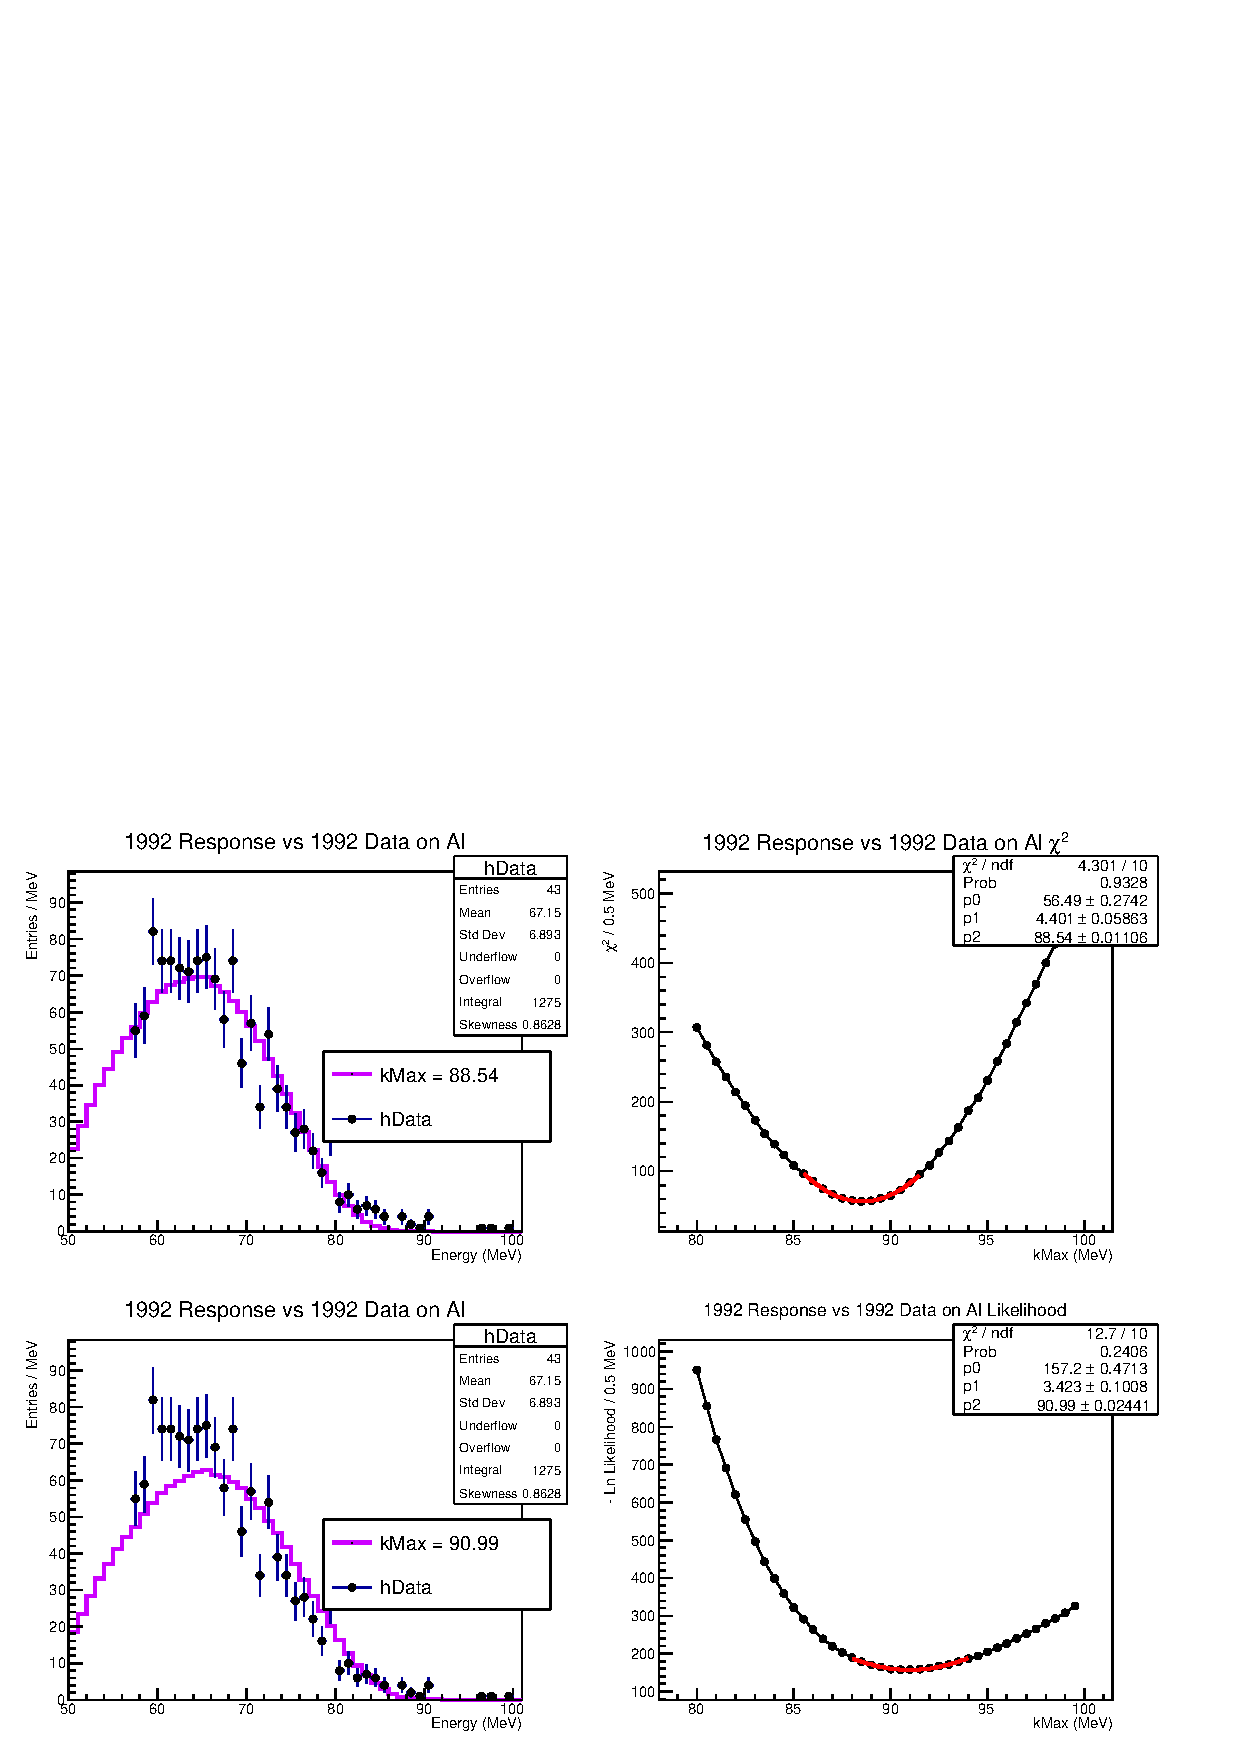
\includegraphics[width=0.8\linewidth]{figures/png/1992_resp_1992_Al_data_allPlots_singleK.png}
  \caption{The left figures show the best fit convolved closure approximation spectrum. The right figures
  show the parabolic fit to find the best fit endpoint energy. The top figures use $\chi ^2$ 
  minimization while the bottom figures use $\mathcal{L}$ minimization.}
  \label{fig:1992AlFits}
\end{figure}


\begin{figure}[h]
  \centering
  \subfloat[ $\chi^2$ Minimization Fit \label{fig:ChiSq}]{%
  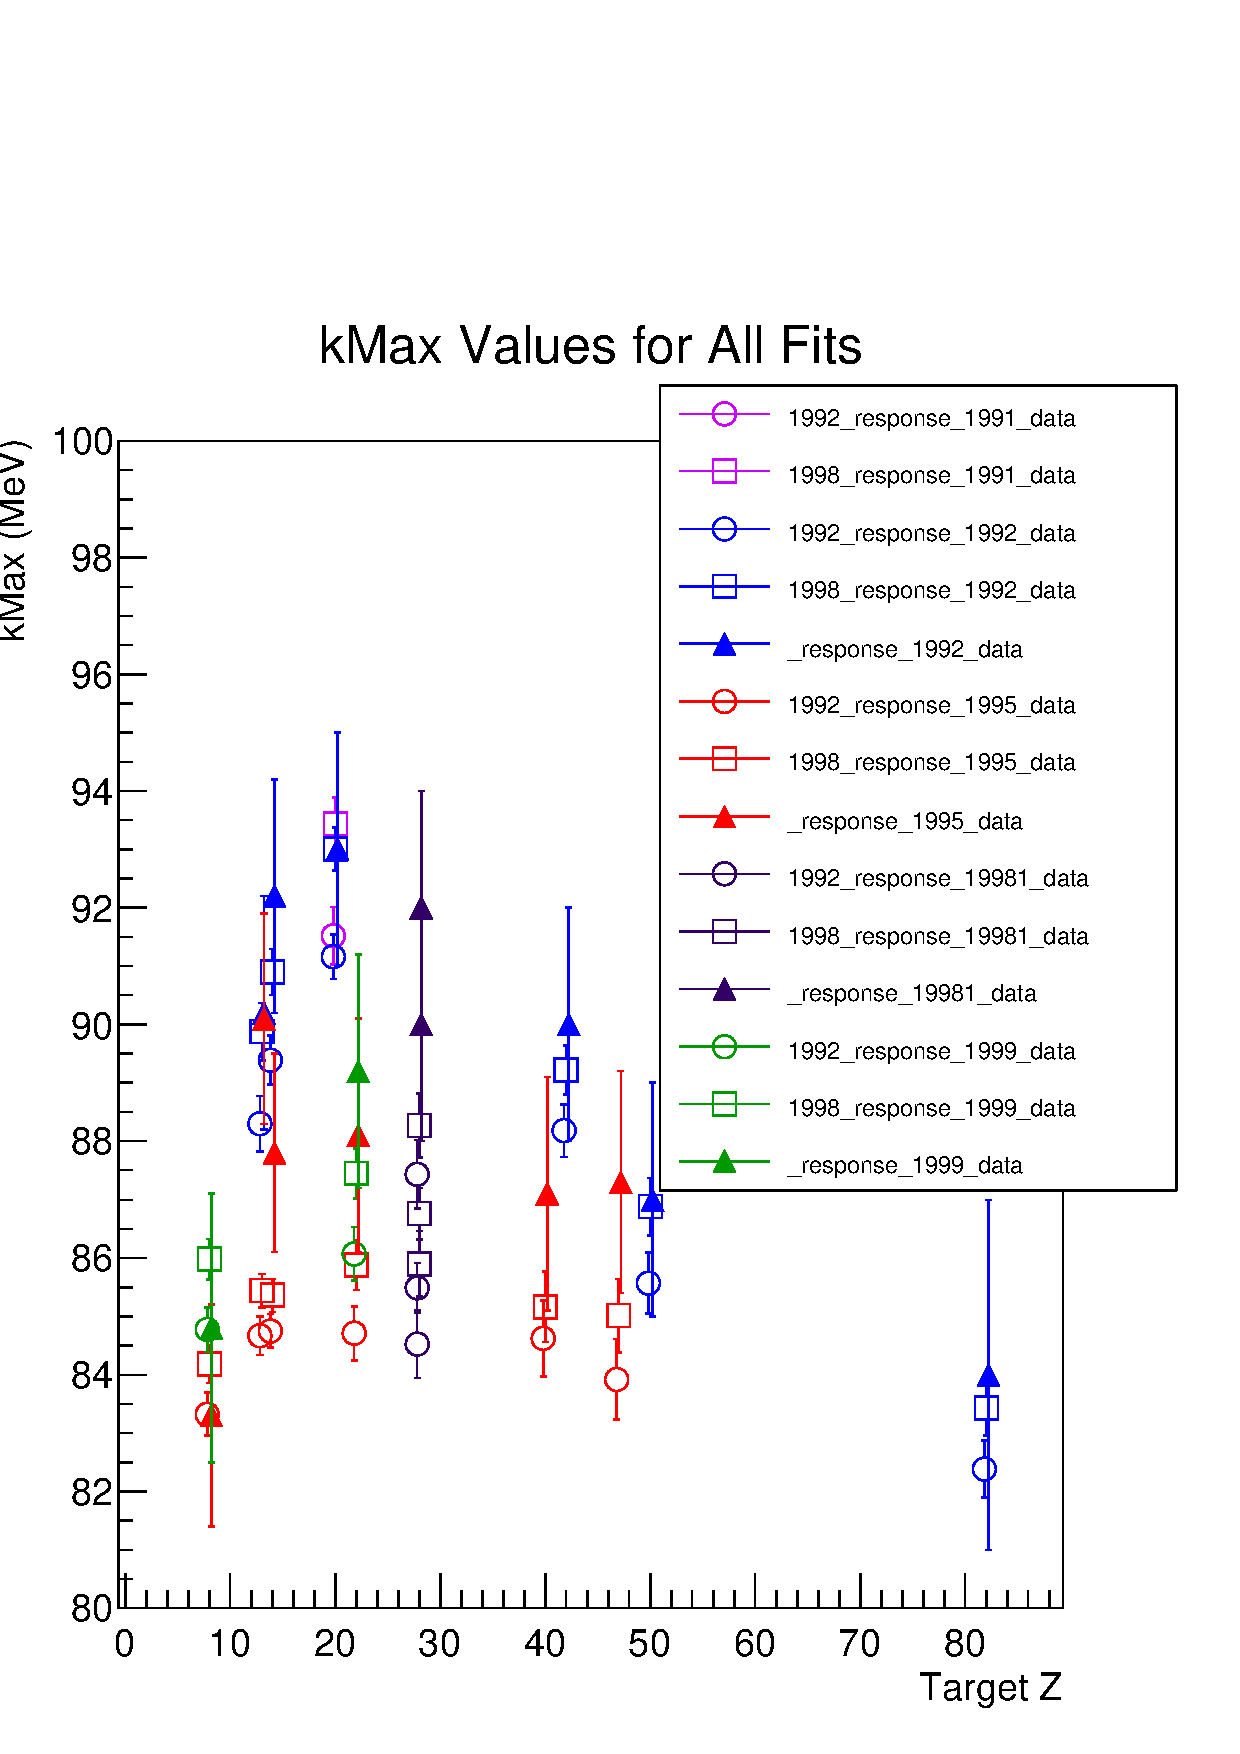
\includegraphics[width=0.48\linewidth]{figures/png/all_kMaxesChiSq_vs_target_z.png}
  }
  \hfill
  \subfloat[$\mathcal{L}$ Minimization Fit  \label{fig:NLL}]{%
  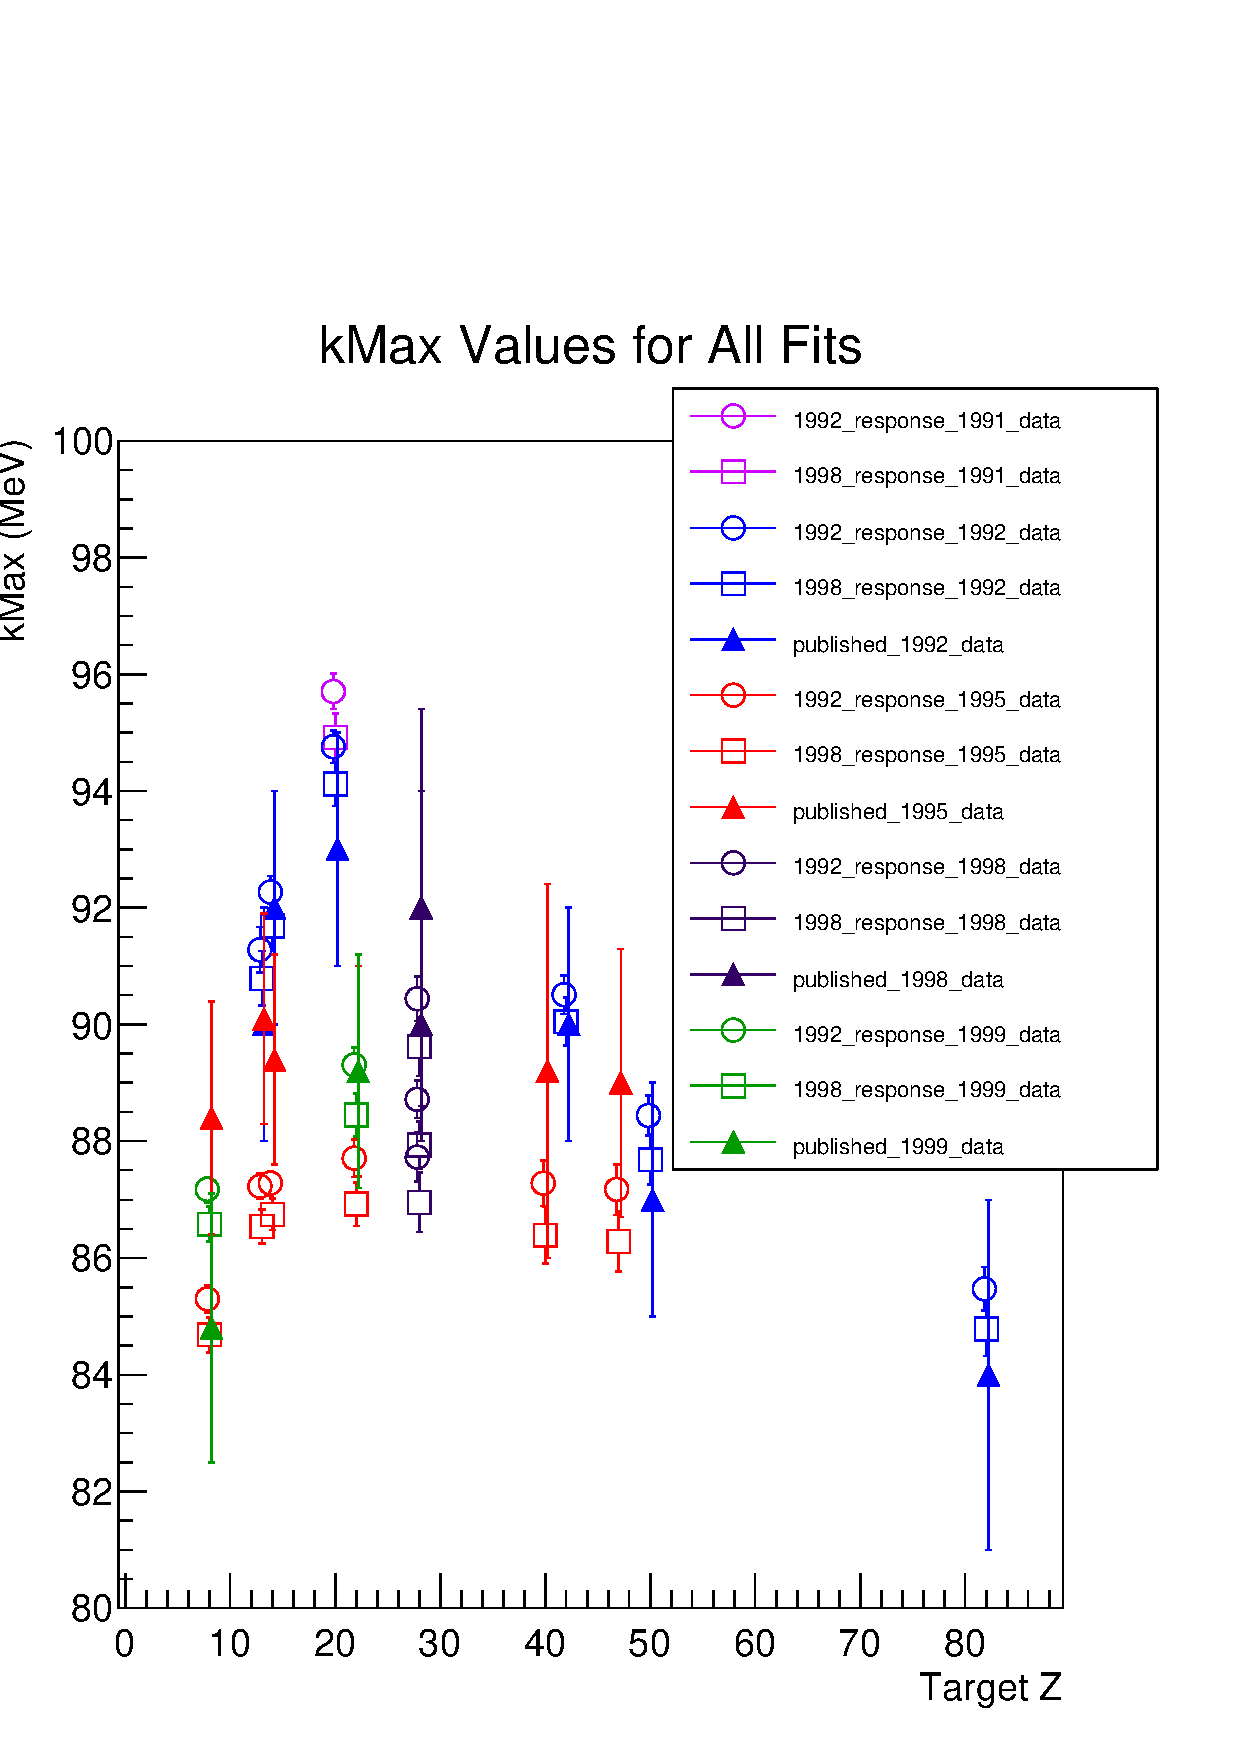
\includegraphics[width=0.48\linewidth]{figures/png/all_kMaxesNLL_vs_target_z.png}
  }
  \caption{Fit results vs target Z using (a) $\chi^2$ minimization and (b) $\mathcal{L}$ minimization.
    The 1992 detector response function data points (circles) are offset by -0.2 in z and the published data points (triangles)
    are offset by +0.2 in z.
  }
\end{figure}

%%%%%%%%%%%%%%%%%%%%%%%%%%%%%%%%%%%%%%%%%%%%%%%%%%%%%%%%%%%%%%%%%%%%%%%%%%%%%%%%%%%%%%%%%%%%%%%%%%%%%%
%% Should we include the chi square of the NLL fits, if we're not sure how they're defined in ROOT? %%
%%%%%%%%%%%%%%%%%%%%%%%%%%%%%%%%%%%%%%%%%%%%%%%%%%%%%%%%%%%%%%%%%%%%%%%%%%%%%%%%%%%%%%%%%%%%%%%%%%%%%%

\begin{figure}[h]
  \centering
  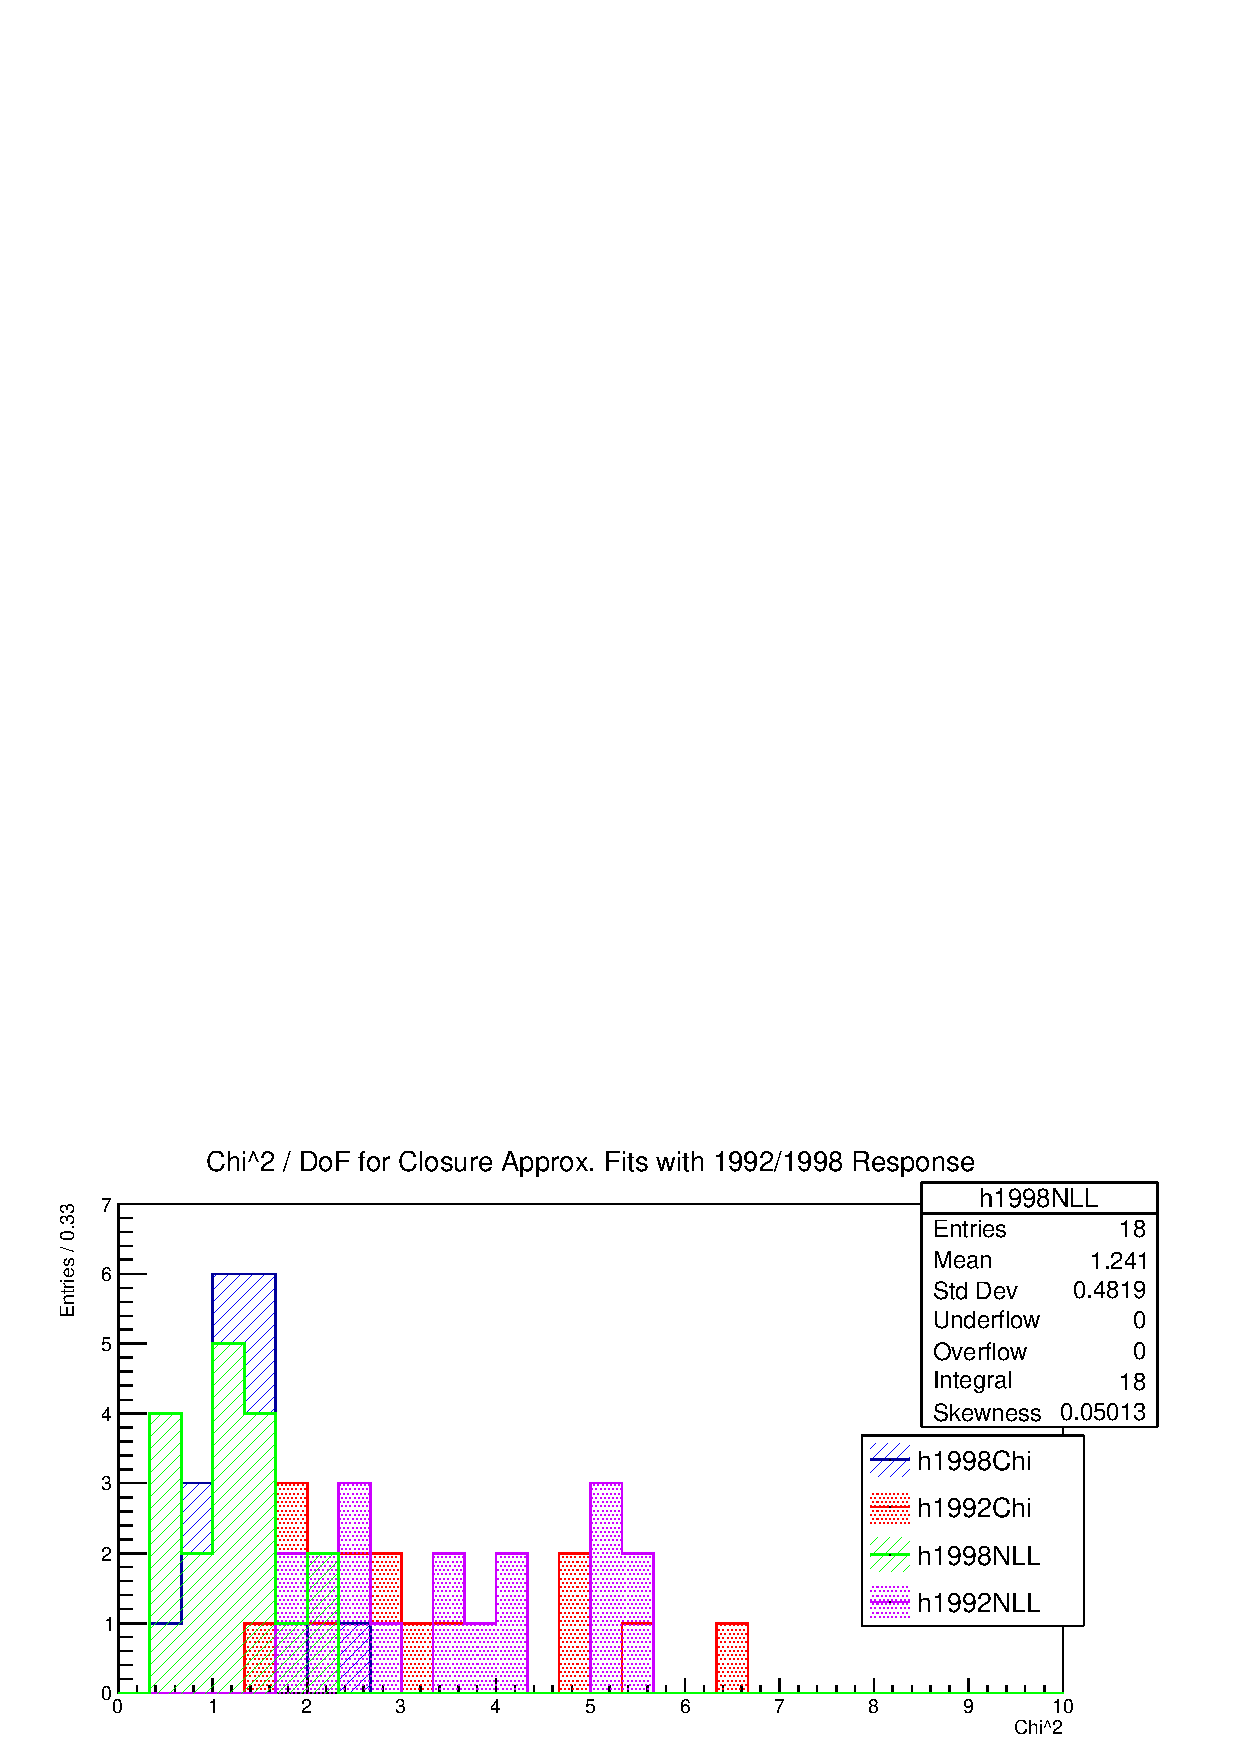
\includegraphics[width=0.8\linewidth]{figures/png/chiSq_of_fits.png}
  \caption{Fit $\chi^2$ values for both detector response functions and both fitting methods. }
  \label{fig:ChiSqOfFits}
\end{figure}


\begin{figure}[h]
  \centering
  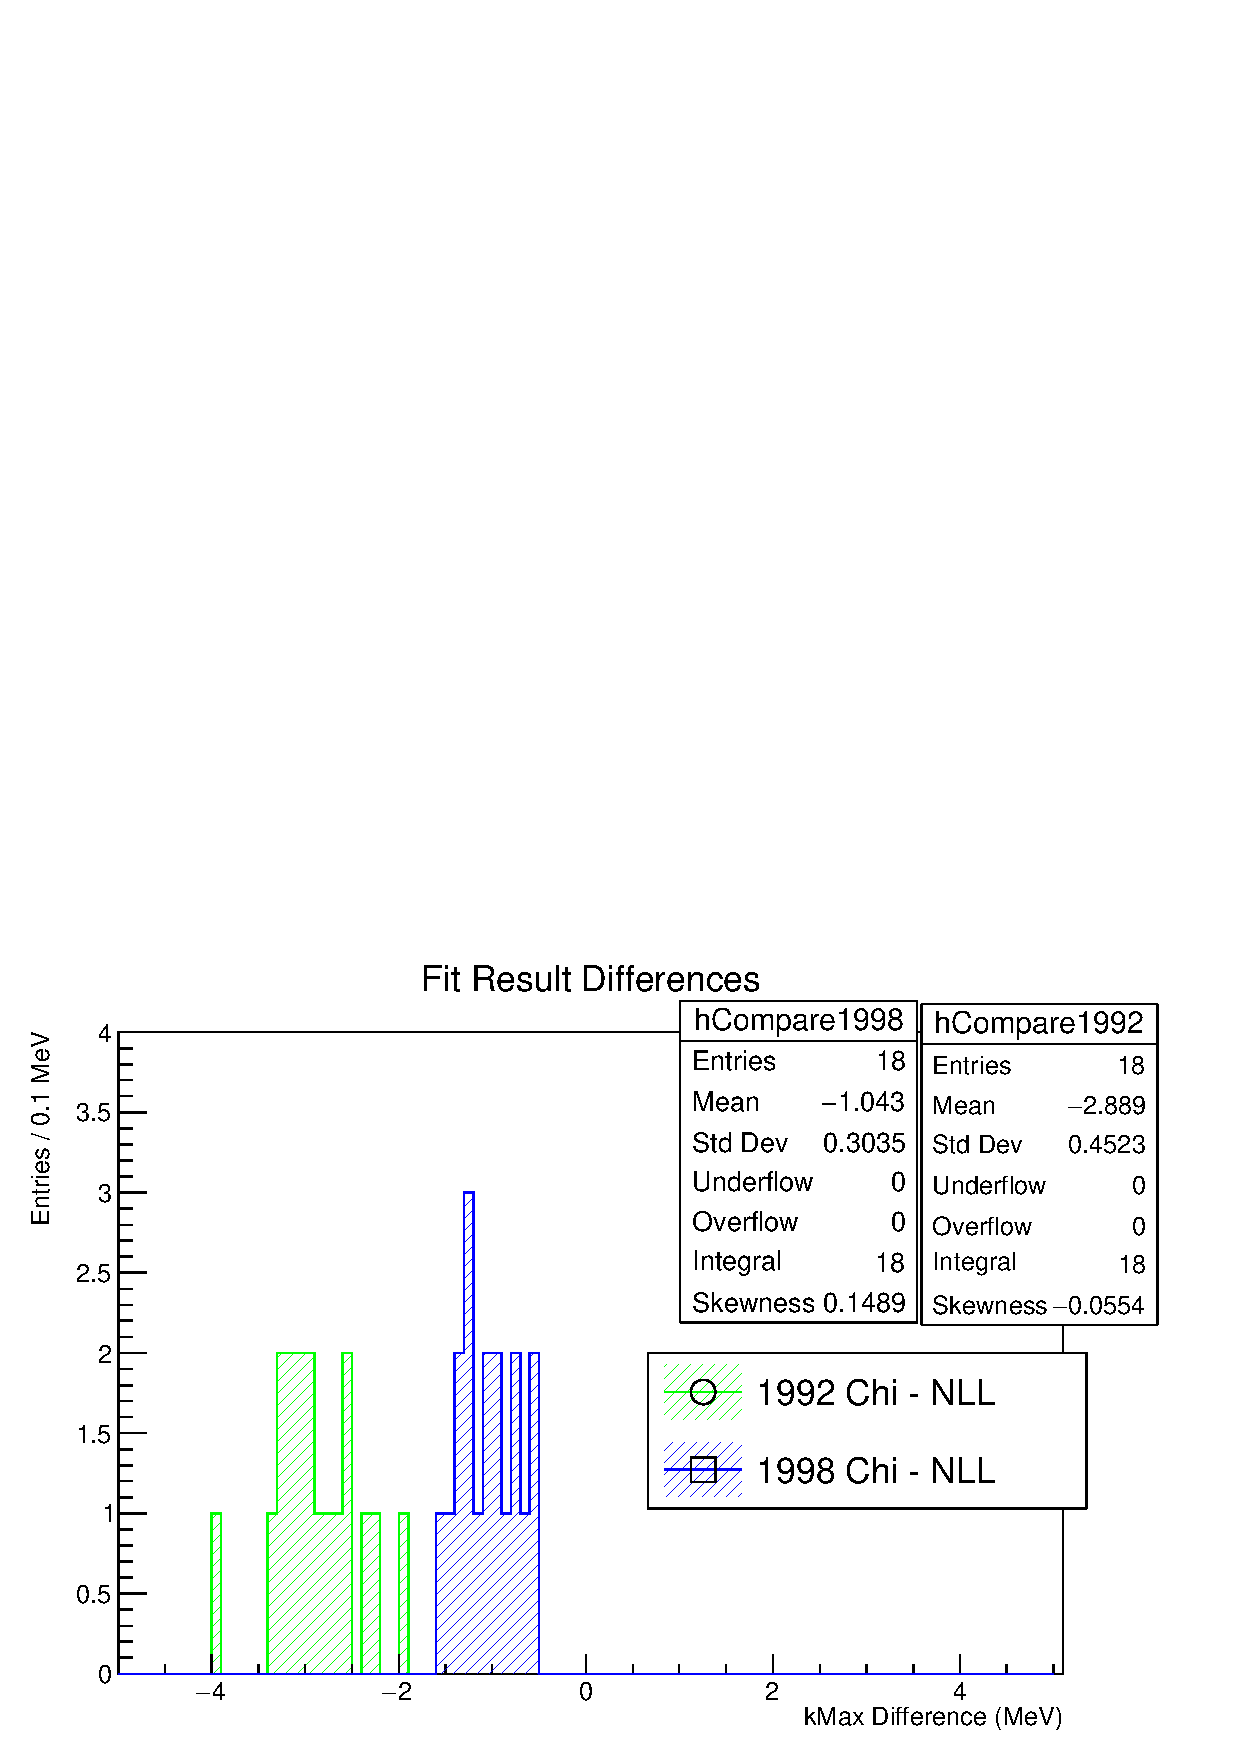
\includegraphics[width=0.8\linewidth]{figures/png/compare_fit_results_92_v_98_unrestrictedOnly.png}
  \caption{The difference between the $\kmax$ values found using $\chi^2$ and
    $\mathcal{L}$ minimization using the 1992 and 1998 detector response functions.}
  \label{fig:compareFits}
\end{figure}

\begin{figure}[h]
  \centering
  \subfloat[ 1992 detector response \label{fig:1992ToyErrs}]{%
  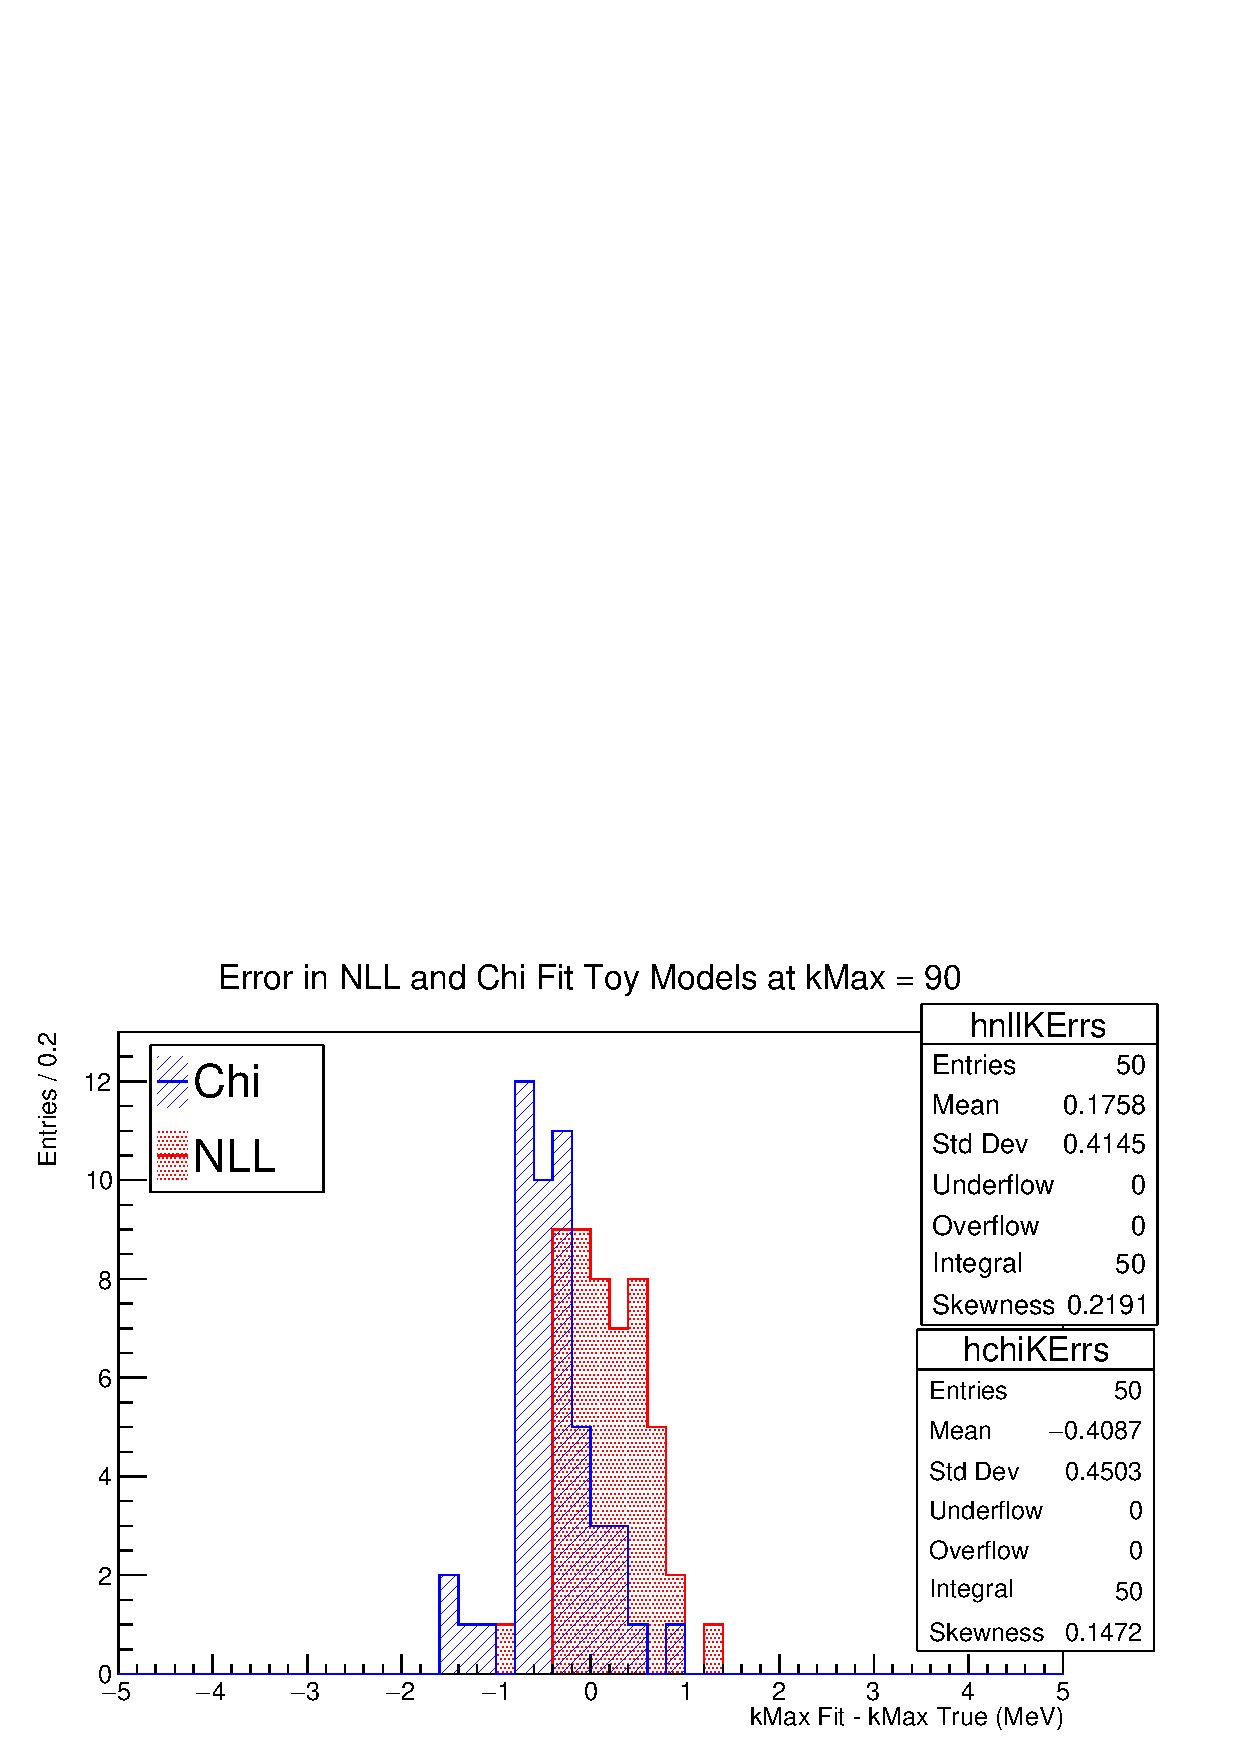
\includegraphics[width=0.48\linewidth]{figures/png/toy_kMax_errors_1992_response.png}
  }
  \hfill
  \subfloat[ 1998 detector response  \label{fig:1998ToyErrs}]{%
  \includegraphics[width=0.48\linewidth]{figures/png/toy_kMax_errors_1998_response.png}
  }
  \caption{Distributions for the fit bias $\Delta{K_{max}} = K_{max}^{fit}-K_{max}^{true}$ for 50 toy %
    data sets using the (a) 1992 or (b) 1998 detector response function.
    The toy data sets are generated from a convolution with an endpoint energy of 90 MeV
    and generated with 1275 data points.
  }
  \label{fig:ToyFitErrs}
\end{figure}

\begin{figure}[h]
  \centering
  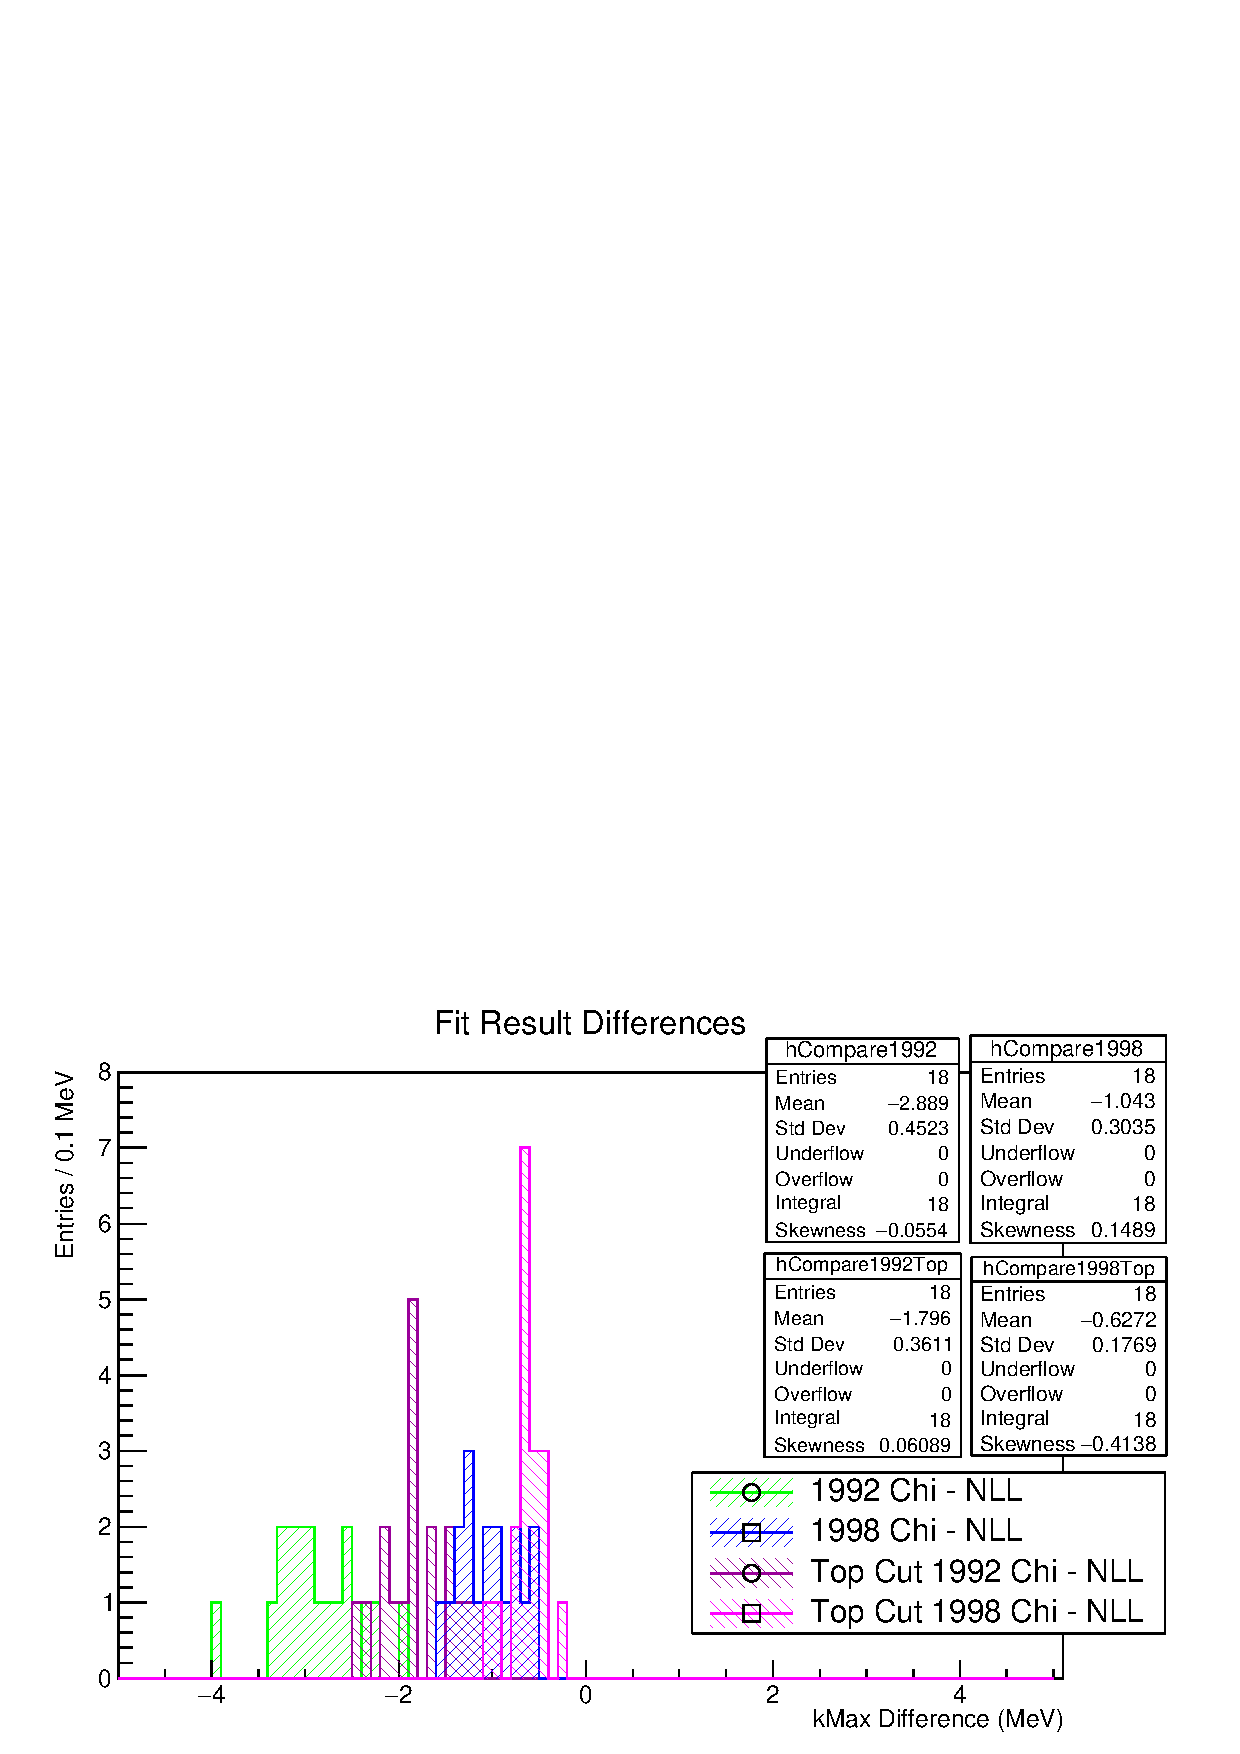
\includegraphics[width=0.7\linewidth]{figures/png/compare_fit_results_92_v_98_with_topCut.png}
  \caption{The difference between the $\kmax$ values found using $\chi^2$ and
    $\mathcal{L}$ minimization with and without excluding the top 0.5\% of the data
    using the 1992 and 1998 detector response functions.}
  \label{fig:compareFitsTopCut}
\end{figure}


%% \begin{figure}[h]
%%   \centering
%%   \subfloat[ 1992 detector response \label{fig:1992ToyZs}]{%
%%   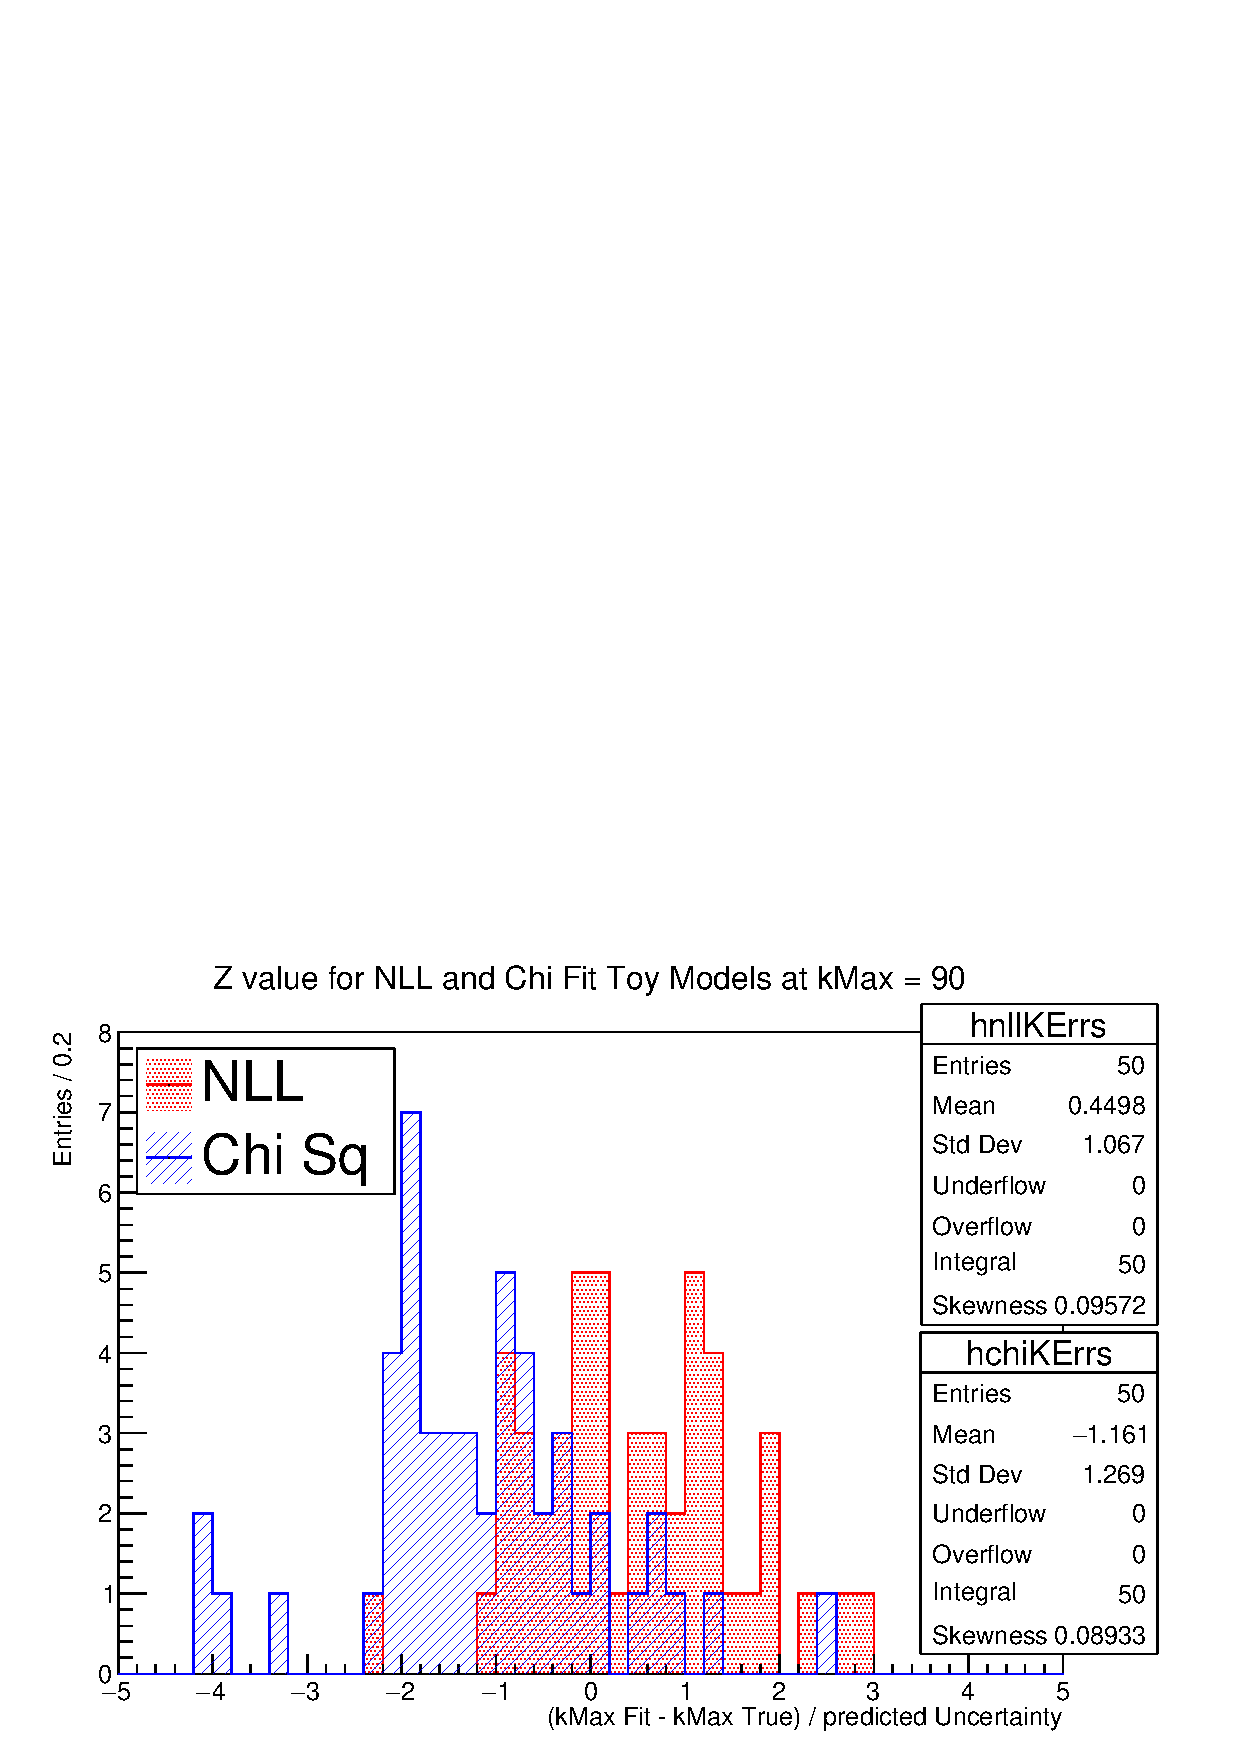
\includegraphics[width=0.48\linewidth]{figures/png/toy_kMax_z_values_1992_response.png}
%%   }
%%   \hfill
%%   \subfloat[ 1998 detector response  \label{fig:1998ToyZs}]{%
%%   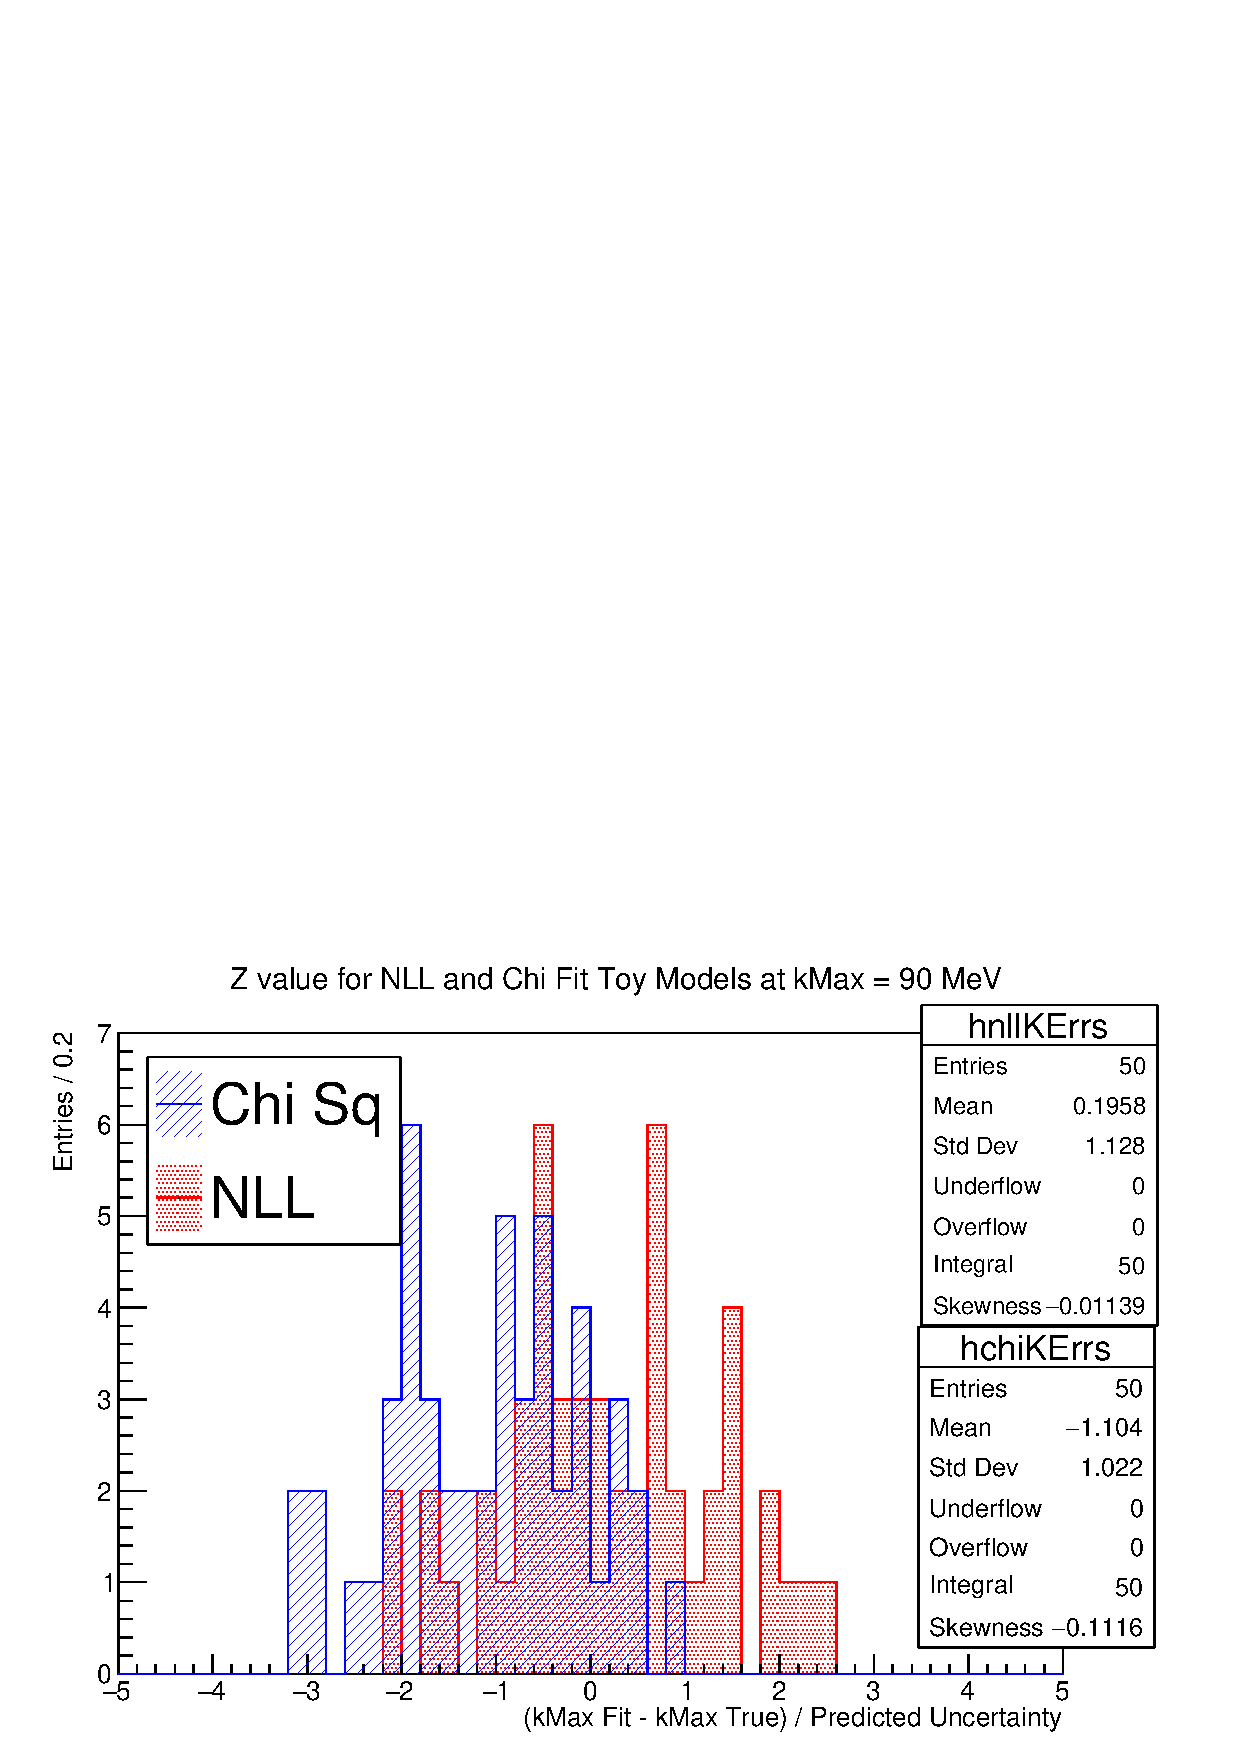
\includegraphics[width=0.48\linewidth]{figures/png/toy_kMax_z_values_1998_response.png}
%%   }
%%   \caption{Fit results z values for 50 toy data sets using the (a) 1992 or (b) 1998 detector response function.
%%     The toy data sets are generated from a convolution with an endpoint energy of 90 MeV and generated
%%     with 1275 data points. The z value for a fit is the fit endpoint value minus the true value, divided
%%     by the fit estimated uncertainty. 
%%   }
%%   \label{fig:ToyFitZs}
%% \end{figure}




%%%%%%%%%%%%%%%%%%%%%%%%%%%%%%%%%%%%%%%%%%%%%%%%%%%%%%%%%%%%%%%%%%%%%%%%%%%%%%%
\section { Discussion }
There are several interesting results that have come out of this study, as well as several
questions raised. We find that our fits result in significantly
smaller errors on $\kmax$ than the published ones. It seems very likely that the TRIUMF 
RMC spectrometer collaboration used the wrong definition of the fit errors. The plot on 
page 45 of reference \cite{RMC_1995_Bergbusch_MS_thesis}, shown in figure \ref{fig:BergbuschChiSq}, 
indicates that the fit error has been defined as the change in the parameter value
corresponding to the change in the fit $\chi^2$/DOF by one, rather than the change
by one in the total fit $\chi^2$. The number of bins in the fit histograms
is about 35-40, which agrees with our fit errors being 5-6 times smaller than
the published ones.


  \begin{figure}[h]
    \centering
    \includegraphics[width=0.8\linewidth]{figures/png/Bergbusch_O16_chisq_plot.png}
    \caption{Figure shown on page 45 from reference \cite{RMC_1995_Bergbusch_MS_thesis} showing
    how the fit error is defined for the fit of the $^{16}$O RMC data. }
    \label{fig:BergbuschChiSq}
  \end{figure}

The 1998 parameterization of the detector response gives significantly better
fits of all spectra published by the TRIUMF RMC spectrometer (1992 \cite{RMC_1992_PhysRevC.46.1094},
1995 \cite{RMC_1995_Bergbusch_MS_thesis}, 1998 \cite{RMC_1998_PhysRevC.58.1767}, and 
1999 \cite{RMC_1999_PhysRevC.59.2853}).
The $\chi^2$ of the fits with 1992 parameterization of the detector response are large enough
to suggest the wrong parameterization. Our $\chi^2$ per degree of freedoms are consistent with
the published ones using the 1998 detector response.

However, the 1992 detector response is consistent with the positon and the width of the 
RPC peak published in 1992, while 1998 response is not. 
This confirms internal inconsistency in the 1992 publication.

Lastly, fit $\kmax$ values for the same target in different years vary on a scale large compared
to the fit errors. This shows inconsistency between the different publication years despite
no change in the detector reported in the published works.

% \newpage
%%%%%%%%%%%%%%%%%%%%%%%%%%%%%%%%%%%%%%%%%%%%%%%%%%%%%%%%%%%%%%%%%%%%%%%%%%%%%%%
\section{ Summary }

The only claim we can confidently make is that the fit uncertainties on $\kmax$ are
of the order of 0.5 MeV, not 2 MeV. Published uncertainties of about 2-3 MeV
have been derived using the wrong procedure (fit of the distribution of $\chi^2$/DOF
instead of the total $\chi^2$ as a function of the parameter). To fully understand the RMC background at Mu2e,
Mu2e will need to measure $\kmax$ for the stopping target material used.


For the planned stopping target material, aluminum, the fit results for $\kmax$ are consistent with 
the published results - around 90 MeV. For background studies at Mu2e, the suggest plan is to use
the published endpoint value for aluminum from TRIUMF, 90 MeV, with an estimated error of 
$\pm 0.5$ MeV. For background estimates, an analysis should be performed using
$\kmax = 90$ MeV and $\kmax + 3\sigma = 91.5$ MeV.


%% Plan : use aluminum data

%% a)Assume $90 \pm 0.5$ MeV, determine the RMC background

%% b) assume kMax + 3 sigma, determine the RMC background

%%%%%%%%%%%%%%%%%%%%%%%%%%%%%%%%%%%%%%%%%%%%%%%%%%%%%%%%%%%%%%%%%%%%%%%%%%%%%%% 
% \section{ Acknowledgements }
% 
% We want to thank ...
% 
%%%%%%%%%%%%%%%%%%%%%%%%%%%%%%%%%%%%%%%%%%%%%%%%%%%%%%%%%%%%%%%%%%%%%%%%%%%%%%
     %% 
     %% % \addcontentsline{toc}{chapter}{Bibliography}
     %
\bibliographystyle{plain}
\bibliography{radiative_muon_capture}

\appendix
%% \appendixpage

\input{fit_results}

% \printbibliography
\end{document}


% ------------------------------------------------------------------------------
% templates
% ------------------------------------------------------------------------------
% Table ~\ref{table:summary} gives summary the numbers used in this study.
% 
% \hspace{-0.1in}
% \begin{table}[htbp]
%   \label{table:summary}
%   \begin{center} 
%     {\renewcommand{\arraystretch}{1.0}   % change 1.0 to 1.1 to increase the spacing between the table lines
%       \begin{tabular}{|c|c|c|c|}
%         \hline
%                             & default TS geometry & misaligned TS geometry   &  Ratio(default/misaligned)    \\ 
%         \hline
%         $N_{POT}$            &  $4.96 \cdot 10^6$  &    $5.00 \cdot 10^6$      &   0.992   \\ 
%         $N_{\mu}^{TS3u}$      &  65648              &     61354                 &   1.070   \\ 
%         $N_{\mu}^{TS5}$       &  28517              &     27351                 &   1.043   \\ 
%         $N_{\mu}^{ST}$        &  8868               &      8396                 &   1.056   \\ 
%         $N_{\mu}^{ST}/N_{POT}$ &  $1.79 \pm 0.02$    &    $1.68 \pm 0.02$        &   $1.065 \pm 0.03$        \\ 
%         \hline
%       \end{tabular}
%     }
%   \end{center}
%   \caption{
%     Muons rates at different points of the Mu2e beamline and stopping muon rates for nominal and 
%     misaligned TS geometries
%   }
%   % \vspace{0.5in}
% \end{table}
